
% NIM A / Elsevier first manuscript draft
% Compile with: pdflatex balloon511_nima_draft_en.tex
% For submission, replace placeholder authors/affiliations and move Highlights to Elsevier's separate highlights file if requested.

\documentclass[preprint,12pt]{elsarticle}

\usepackage{amsmath,amssymb}
\usepackage{booktabs}
\usepackage{graphicx}
\usepackage{hyperref}
\usepackage{xcolor}

\journal{Nuclear Instruments and Methods in Physics Research Section A}
\biboptions{numbers,sort&compress}

\newcommand{\keV}{\,\mathrm{keV}}
\newcommand{\MeV}{\,\mathrm{MeV}}
\newcommand{\cms}{\,\mathrm{cm^{-2}\,s^{-1}}}
\newcommand{\cps}{\,\mathrm{s^{-1}}}
\newcommand{\wii}{W2}
\newcommand{\aeff}{A_{\mathrm{eff}}}
\newcommand{\fzero}{F_{0}}
\newcommand{\fthree}{F_{3\sigma}}

\begin{document}

\begin{frontmatter}

\title{Background and 511 keV line sensitivity of a balloon-borne TES Laue-lens telescope\tnoteref{t1}}
\tnotetext[t1]{First full-manuscript draft prepared for a NIM A style submission. Numerical results should be rechecked against the final repository validation outputs before submission.}

\author[inst1]{Author list to be completed}
\address[inst1]{Institution list to be completed}

\begin{abstract}
The Galactic 511 keV annihilation line is a direct tracer of low-energy positrons, but its compact-source content and narrow-line kinematics remain difficult to measure because MeV instruments are strongly background dominated. We present a full-chain Monte Carlo and rate-folding study for a balloon-borne pointed 511 keV telescope that combines a Ge(111) Laue lens with a transition-edge-sensor (TES) microcalorimeter focal plane. The model couples the focused optical phase space to an engineering detector/cryostat geometry, prompt atmospheric backgrounds, activation buildup, exact-position delayed-source transport, active-shield vetoes, Compton/field-of-view consistency cuts, a narrow line window, and mission-time rate variation. The nominal exact-position chain uses a 10 m focal-length Laue configuration with $\aeff(511\keV)=20.08476\,\mathrm{cm^2}$, 50,000 equal-activity delayed-source support elements, and a $510.58$--$511.42\keV$ analysis window. At a reference point-source flux of $10^{-4}\,\mathrm{ph\,cm^{-2}\,s^{-1}}$, the selected line-window background and signal rates are $0.0629804\cps$ and $0.00118117\cps$, respectively. The mission-time fold gives $Z_{20\mathrm{d}}=6.13039$, a $3\sigma$ detection time of $4.77766$ d, a 20-d $3\sigma$ flux threshold of $4.89365\times10^{-5}\cms$, and a 1 Ms threshold of $6.35099\times10^{-5}\cms$. A transport-backed exact-position support-size and seed sweep changes the total line-window background by only 1.119\% and $Z_{20\mathrm{d}}$ by 0.551\%. We also report secondary spatial-analysis and atmospheric-line-of-sight checks, while keeping the hard-window exact-position chain as the primary rate calculation. The results indicate that focused TES spectroscopy can reach scientifically useful narrow-line sensitivity from a balloon platform, provided activation and prompt atmospheric backgrounds are modeled in the same detector-coupled selection space as the signal.
\end{abstract}

\begin{keyword}
Gamma-ray instrumentation \sep 511 keV annihilation line \sep transition-edge sensors \sep Laue lens \sep balloon-borne telescope \sep Monte Carlo background simulation \sep activation background
\end{keyword}

\end{frontmatter}

% Highlights for Elsevier submission system, to be placed in a separate file if required:
% - Detector-coupled background model for a balloon-borne focused 511 keV TES telescope.
% - Exact-position delayed activation is transported through the same line-window selection as the focused signal.
% - The hard-window exact-position chain gives F_3sigma(20 d)=4.89e-5 ph cm^-2 s^-1.
% - Transport-backed M/seed convergence stabilizes the final W2 significance at the sub-percent level.

\section{Introduction}
\label{sec:intro}

The 511 keV gamma-ray line from electron--positron annihilation is one of the cleanest spectroscopic signatures of antimatter in the Galaxy. After positrons slow down in the interstellar medium, they annihilate either directly with electrons, producing two photons near 511 keV, or through positronium formation, producing the 511 keV line together with a three-photon continuum below the line. This radiative complex probes positron production, propagation, thermalization, and annihilation conditions \cite{Prantzos2011}. The line was first reported from the Galactic-center direction by balloon-borne experiments and later identified unambiguously with high-resolution Ge detectors as positron-annihilation radiation \cite{Prantzos2011}. The observed Galactic flux implies a positron annihilation rate of order $10^{43}\,\mathrm{e^+\,s^{-1}}$, making the origin of these positrons a long-standing problem in MeV gamma-ray astronomy \cite{Prantzos2011,Kierans2020}.

The candidate source classes span standard and non-standard physics. Conventional astrophysical candidates include $\beta^+$ decay of radioisotopes synthesized in massive stars, novae, core-collapse supernovae, and thermonuclear supernovae; pair creation in compact objects such as X-ray binaries, microquasars, pulsars, and the Galactic-center black hole; and cosmic-ray interactions \cite{Prantzos2011,Siegert2016AA}. More speculative explanations include light dark matter decay or annihilation and hidden-sector scenarios \cite{Prantzos2011,Yoneda2025}. The difficulty is that the observed annihilation morphology is shaped not only by where positrons are produced, but also by how far they propagate before thermalization and annihilation. Spectroscopy constrains the annihilation medium through the line centroid, line width, and positronium fraction, while continuum limits above 511 keV constrain the injection energy \cite{Prantzos2011,Siegert2016AA}. The most discriminating observables for source identification---compact-source content, small-scale structure, velocity shifts, and spatially resolved line broadening---remain limited by instrumental sensitivity, angular resolution, and background systematics.

The current observational picture has been shaped by OSSE/CGRO, INTEGRAL/SPI, and COSI. INTEGRAL/SPI established a bright bulge-like component and fainter disk emission, with the detailed bulge/disk decomposition depending on the adopted sky model and instrumental-background treatment \cite{Siegert2016AA,Yoneda2025}. Recent long-exposure SPI analyses recover the central, broad-bulge, and disk structures and suggest marginal additional structures associated with massive-star regions \cite{Yoneda2025}. COSI provided an important independent measurement from a 46-d super-pressure-balloon flight, detecting the Galactic 511 keV signal with Compton imaging and finding that the emission is broader than a single point source \cite{Kierans2020,Siegert2020COSI}. These results demonstrate both the scientific value and the practical difficulty of MeV line astronomy: the celestial line is weak, while atmospheric and instrumental backgrounds are strong and time dependent.

Wide-field Compton telescopes are essential for mapping the large-scale 511 keV sky. A complementary strategy is to use a pointed telescope that concentrates 511 keV photons onto a small, high-resolution focal plane. A pointed system is especially useful for testing whether a fraction of the annihilation luminosity is produced by unresolved point sources, a bright central core, or transient pair-plasma episodes in compact objects. This motivation is reinforced by annihilation signatures reported during the 2015 outburst of V404 Cygni, which indicate that accreting stellar-mass black holes can produce pair plasma at astrophysically relevant rates \cite{Siegert2016V404}. Such a payload does not replace wide-field Compton missions; it addresses a different observable in a narrower field of view.

The 511-CAM concept follows this route by combining gamma-ray concentrating optics with stacked transition-edge-sensor microcalorimeter arrays \cite{Shirazi2023}. It is attractive because it joins photon concentration with sub-keV calorimetric energy resolution, two capabilities rarely available together at MeV energies. A projected 511 keV detector-assembly resolution of a few $10^2$ eV FWHM corresponds to a velocity scale of a few $10^2\,\mathrm{km\,s^{-1}}$ and could enable velocity-shift or line-broadening measurements in favorable cases \cite{Shirazi2023}. Event topology also matters. Single-pixel photoelectric events provide the cleanest spectroscopy, while multi-pixel events can be checked against Compton kinematics and rejected if inconsistent with photons arriving through the focusing optics.

The central technical challenge is background. Balloon-borne gamma-ray spectrometers operate in a strong radiation environment and are necessarily background dominated. Classical studies of balloon-borne Ge spectrometers identify atmospheric-neutron scattering, atmospheric and cosmic gamma-ray aperture flux, beta decays of activation products, and shield leakage as major background components; they also emphasize minimizing passive material near the detector and lowering effective shield thresholds where possible \cite{Gehrels1985}. For a 511 keV line payload, the problem is sharper because the science signal lies at the same energy as strong atmospheric and instrumental annihilation features. A credible sensitivity estimate therefore requires a detector-coupled model of the optics, entrance windows, cryostat, passive material, active shield, prompt atmospheric components, and delayed activation.

Detailed Monte Carlo mass modeling is the standard route to such estimates. The INTEGRAL/SPI response production required a high-fidelity mass model, ground- and in-flight-calibration comparisons, and a practical separation between imaging response and redistribution response to control computing and storage costs \cite{Sturner2003}. Modern MeV mission studies, including AMEGO and COSI, similarly rely on Geant4/MEGAlib-based simulations to calculate response, background, event reconstruction, and sensitivity \cite{Agostinelli2003,Zoglauer2006,Caputo2017,Karwin2023,Gallego2025}. The same philosophy is adopted here, but applied to a narrower and more demanding target: a balloon-borne, focused, narrow-line 511 keV telescope with a TES focal plane.

This paper presents a detector-coupled simulation and sensitivity study for such a payload. The simulation chain starts from a Ge(111) Laue-lens source model at 511 keV and transports focused photons through the detector entrance window into an engineering detector/cryostat mass model. The modeled assembly includes the TES focal plane, staged thermal windows, a Be entrance window, Cu/W passive shielding, cryogenic service proxies, and an active CsI shield. The background chain includes prompt atmospheric components, activation buildup, exact-position delayed-source transport, active-shield vetoes, Compton/field-of-view consistency cuts, a narrow 511 keV line window, mission-time rate evolution, and counting-significance estimates. The main contribution is not an isolated effective-area estimate, but a closed rate calculation in which signal and background pass through the same detector-coupled selection definitions.

The remainder of the paper is organized as follows. Section~\ref{sec:requirements} summarizes the science-driven instrument requirements. Section~\ref{sec:workflow} describes the simulation chain. Sections~\ref{sec:geometry}--\ref{sec:selection} describe the detector geometry, optics bridge, background model, and event selections. Section~\ref{sec:results} presents the sensitivity, convergence, and background-composition results. Section~\ref{sec:discussion} discusses interpretation, limitations, and future work. Section~\ref{sec:conclusions} summarizes the main conclusions.

\section{Science and instrument requirements}
\label{sec:requirements}

The instrument considered here is optimized for a pointed, narrow-line measurement rather than all-sky imaging. The primary science case is the detection or exclusion of compact 511 keV emission at fluxes of order $10^{-4}\cms$ or below during a long-duration balloon exposure. This flux scale is motivated by the need to test bright central-core, compact-source, and transient pair-plasma scenarios while remaining complementary to wide-field Compton surveys.

The requirements are stated at the level needed for the present simulation, not as final flight-system specifications. They define what the model must preserve for a credible rate claim: the source flux normalization, the focused entrance phase space, the narrow line-window response, and the same detector selection for signal and background. This distinction is important because several quantities, including the TES energy response and final cryostat layout, remain design assumptions or engineering proxies.

Four requirements follow. First, the telescope must concentrate 511 keV photons so that a small focal plane can be used without sacrificing collecting area. Second, the focal-plane response must support a sub-keV analysis window so that the line-window background scales with a narrow spectral interval rather than a broad MeV-band continuum. Third, the detector and shield model must suppress atmospheric, activation, and side-entry backgrounds while explicitly accounting for passive material near the TES absorbers. Fourth, the simulation chain must treat prompt background, delayed activation, focused signal, vetoes, event topology, and mission-time variation consistently. Table~\ref{tab:requirements_traceability} summarizes how these requirements map onto the baseline exact-position implementation.

\begin{table}[t]
\centering
\caption{Traceability from science drivers to instrument and simulation requirements. The table summarizes requirements used to define the baseline exact-position analysis; it is not a separate sensitivity calculation.}
\label{tab:requirements_traceability}
\footnotesize
\begin{tabular}{@{}p{0.20\linewidth}p{0.22\linewidth}p{0.35\linewidth}p{0.14\linewidth}@{}}
\toprule
Science driver & Requirement & Current implementation or evidence & Workflow component \\
\midrule
Compact 511 keV targets at $\sim10^{-4}\cms$ or below & Concentrate 511 keV photons onto a small focal plane & 10 m Ge(111) Laue lens with $\aeff(511\keV)=20.08476\,\mathrm{cm^2}$; tracked focal particles passing the Be entrance aperture are replayed through the detector model & Laue optics; detector coupling \\
Narrow-line spectroscopy rather than broad-band counting & Use a sub-keV analysis window and preserve source-flux normalization & $\wii=510.58$--$511.42\keV$; selected signal $0.00118117\cps$ at $\fzero=10^{-4}\cms$; source-flux response $11.8117\,\mathrm{cps}/(\mathrm{ph\,cm^{-2}\,s^{-1}})$ & Detector selection; source normalization \\
Balloon prompt, side-entry, and activation backgrounds & Apply detector-coupled veto and topology cuts to signal and background streams & CsI post-processing veto, side-entry Compton/FoV consistency, exact-position delayed transport; selected $\wii$ background $0.0629804\cps$ split into prompt $0.0590827\cps$ and delayed $0.00389764\cps$; auxiliary upstream-optics interface closure with matched Ge volume and $1060\,\mathrm{cm}$ source surface & Common detector selection; auxiliary closure \\
Mission-level sensitivity result & Fold rates through mission time and test delayed-source sampling stability & Final cumulative calculation gives $Z_{20\mathrm{d}}=6.13039$ and $\fthree(20\mathrm{d})=4.89365\times10^{-5}\cms$; M/seed sweep changes $Z_{20\mathrm{d}}$ by 0.551\% & Mission-time fold; robustness checks \\
\bottomrule
\end{tabular}
\end{table}


These requirements also set the interpretation of the results. A hard-window sensitivity is the primary claim because it depends only on energy selection, vetoing, topology/FoV consistency, and the mission-time rate fold. Focused-spot and annular secondary analyses test spatial-analysis boundaries, but they do not replace the hard-window requirement until a publication-grade spatial-spectral likelihood and nuisance-background treatment are in place.

\section{Simulation workflow}
\label{sec:workflow}

Figure~\ref{fig:workflow} summarizes the workflow. The calculation is divided into geometry definition, prompt and buildup transport, delayed-source construction, focused-optics transport, detector-coupled signal replay, detector event selection, mission-time rate folding, source-case normalization, and cumulative significance evaluation. The present manuscript uses the baseline position-preserving delayed-source chain as the primary rate calculation. This chain is called ``exact-position'' below: the delayed decays are sampled from the recorded radioactive-production positions instead of being redistributed into an axisymmetric radial profile. The conservative radial-profile delayed-source chain is retained only as a cross-check.

\begin{figure}[t]
\centering
\newcommand{\flowbox}[1]{\fbox{\begin{minipage}{0.17\linewidth}\centering\scriptsize #1\end{minipage}}}
\flowbox{Geometry\\Step00--01}
\(\rightarrow\)
\flowbox{Prompt and buildup\\Step02}
\(\rightarrow\)
\flowbox{Delayed activity\\Step03}
\(\rightarrow\)
\flowbox{Exact-position transport\\Step03}

\vspace{0.8ex}
\(\downarrow\)
\vspace{0.8ex}

\flowbox{Laue optics\\Step04}
\(\rightarrow\)
\flowbox{Optics-detector coupling\\Step09}
\(\rightarrow\)
\flowbox{Detector selection\\Step05}
\(\rightarrow\)
\flowbox{Time fold and significance\\Step06--08}
\caption{Simulation chain used in this work. The important feature is that the focused signal and all background streams are evaluated in the same detector-response and event-selection space before mission-time significance is calculated.}
\label{fig:workflow}
\end{figure}

The primary rate calculation is the baseline exact-position delayed-source chain. It uses full-statistics prompt and activation-buildup transport, a fixed day-15 radionuclide population, sampled equal-activity point-source support elements at recorded production positions, and full downstream propagation through the detector response, event selection, and significance calculation. The older homogeneous-beam and radial-profile delayed-source chains are retained only as cross-checks and are not used for the primary sensitivities.

Table~\ref{tab:simulation_workflow} gives the traceable version of this chain. The labels Step00--Step10 are archive/audit identifiers used to link the paper text to the simulation products; they are not physical terminology. In the manuscript, that internal audit map is compressed into a reproducible method description: each stage has a defined input, a physical or statistical operation, an output consumed by later stages, and an explicit boundary on what may be claimed from it. The optical Monte Carlo is one stage in this chain, not the chain itself. It supplies the Laue-lens effective area and tracked focused phase space; the optics-detector coupling and detector-response chain convert that optical phase space into a detector-coupled point-source sensitivity.

Read as a calculation chain, the steps have different roles. Steps 00--01 freeze the detector mass model and coordinate policy but do not produce a rate. Step02 generates prompt and activation-production histories and defines the exposure normalization. Step03 converts those production histories into a fixed day-15 delayed radioactive population and transports sampled exact-position decays. Step04 is optical only: it computes the focused 511 keV phase space and effective area but contains no detector background. Step09 couples the optical focal-plane phase space to detector transport. Step05 is the first point at which prompt background, delayed background, and focused signal are compared under the same veto, topology, and line-window rules. Steps 06--08 then move from selected rates to mission-time significance. Step10 tests exact-position support size and seed dependence at the final selected-rate level.

The numerical hierarchy used below follows the same logic. Day-15 selected
rates are quoted after the focused signal stream has been scaled by the 10 m
Ge(111) effective area and the reference atmospheric transmission.
Mission-mean rates are quoted from the time-dependent fold, and the primary
$Z$, $T_{3\sigma}$, and flux thresholds are quoted from the cumulative
significance calculation. Exact-position support-size claims are quoted only
after the sampled source has been transported through the same detector
selection and significance chain. This separation avoids mixing unit-injection
rates, day-15 direct expectations, and mission-folded sensitivities in a single
result.

\begin{table}[t]
\centering
\caption{Stepwise simulation workflow used for the baseline exact-position rate calculation. The table is a manuscript-facing compression of the validated workflow; detailed validation files retain the run-level details.}
\label{tab:simulation_workflow}
\begingroup
\setlength{\tabcolsep}{2pt}
\renewcommand{\arraystretch}{0.78}
\tiny
\begin{tabular}{@{}p{0.12\linewidth}p{0.25\linewidth}p{0.36\linewidth}p{0.18\linewidth}@{}}
\toprule
Step & Role in the calculation & Current implementation or evidence & Boundary for interpretation \\
\midrule
00--01 Geometry & Define detector mass model, active volumes, side-entry frame, and injection surfaces & Baseline detector/cryostat geometry: TES array, Be side window, Cu/W passive material, segmented CsI shield; window tilted $45^\circ$ upward & Geometry closure only; not a rate calculation \\
02 Prompt and buildup transport & Generate prompt atmospheric events and activation histories & Detector/cryostat prompt and buildup streams, each with 25,210,216 particles; prompt rates use per-species exposure normalization & Low-stat branches are closure checks; upstream optics mass is outside the primary rate budget \\
03 Delayed activity and source & Convert activation products to a fixed day-15 delayed source & Detector/cryostat delayed activity $85.636696\,\mathrm{Bq}$; nominal exact-position point-source support with $M=50000$ and $10^6$ delayed triggers & Activity preserving; Step10 tests convergence; upstream Ge-proxy delayed activity is a separate side component \\
04 Laue optics & Compute 511 keV effective area and focused focal-plane phase space & Ge(111), 10 m optical Monte Carlo from XOP/CRYSTAL rocking curves; $\aeff(511)=20.08476\,\mathrm{cm^2}$ and spot contained by Be aperture & Signal only; focal crossings are transported 511 keV gammas, not optics self-background \\
09 Optics-detector coupling & Replay tracked optical focal crossings in the detector & Accepted focal gamma rays are written as a MEGAlib particle-list source and transported through the baseline detector setup & Tracked focal crossings only; signal replay does not represent optics self-background \\
Aux. optics hardware & Check upstream-lens prompt/activation boundary & Equal-volume active-Ge lens proxy at 10 m; far-field source radius $1060\,\mathrm{cm}$ from a $1008.8\,\mathrm{cm}$ detector-plus-lens bound; eight EXPACS/PARMA families close prompt and activation-production transport; isolated Ge-proxy delayed transport selects zero W2 events, with a 95\% upper rate $1.25\times10^{-4}\cps$ & Delayed Ge-proxy side component closed; prompt self-background isolation and support hardware remain outside the primary budget \\
05 Detector response & Apply common selection to prompt, delayed, and focused streams & Active-shield post-processing veto, side-entry Compton/FoV consistency, and $\wii$ hard window; day-15 $\wii$ rates $B/S=0.0629804/0.00118117\cps$ & Veto defined by post-processing selection, not production-time trigger filtering \\
06 Mission-time fold & Propagate selected rates through balloon mission time & Time-dependent prompt, delayed activity, atmosphere, and accidental-veto live-factor fold; mean $\wii$ rates $B/S=0.0631923/0.00117281\cps$ & Rate-level fold; no new transport at each time bin \\
07 Source cases & Map detector response to source-flux units & W2 response $11.8117\,\mathrm{cps}/(\mathrm{ph\,cm^{-2}\,s^{-1}})$ for the reference point-source case & Point-source normalization kept separate from diffuse-sky checks \\
08 Significance & Compute cumulative significance and flux thresholds & Hard-window result: $Z_{20\mathrm{d}}=6.13039$, $T_{3\sigma}=4.77766\,\mathrm{d}$, $\fthree(20\mathrm{d})=4.89365\times10^{-5}\cms$ & Gaussian counting metric for consistent comparisons \\
10 Robustness checks & Test support-size and seed dependence at selected-rate level & Four transport-backed cases over $M=5000$, 20,000, and 50,000; W2 background and $Z_{20\mathrm{d}}$ ranges are 1.119\% and 0.551\% & Supports exact-position delayed transport for the primary rates \\
\bottomrule
\end{tabular}
\endgroup
\end{table}


\clearpage

\section{Detector and cryostat mass model}
\label{sec:geometry}

The detector model is an engineering Geant4/MEGAlib proxy mass model for a balloon-borne TES focal-plane assembly mounted at the cold end of a compact dilution-refrigerator (DR) stack \cite{Shirazi2023,Gottardi2021TESReview}. It is not a final flight CAD model, and it is not intended to reproduce the microfabricated TES layers, detailed wiring, readout layout, or every cryogenic service component. Instead, the model preserves the material columns and local apertures that are first-order for 511 keV transmission, scattering, activation, active-shield vetoing, and event topology. The baseline detector/cryostat geometry therefore contains the TES absorber stack, substrate and window proxies, the side Be entrance window, passive shield/collimator material, cryogenic service-mass proxies, and a segmented CsI active anticoincidence shield. Figure~\ref{fig:mass_model} shows the two-dimensional geometry views used as the manuscript-facing mass-model schematic.

The DR and service hardware are represented at proxy-mass level. The model keeps the physical order of the main temperature stages: the TES module is placed at the 50 mK/MXC end, followed by cold-plate and heat-exchanger proxies for the CP, still, 4 K, 60 K, and 300 K service regions. Al shells and windows represent staged radiation shields and the vacuum jacket. Support structures, capillaries, cable bundles, readout boxes, and other services are not laid out as flight-ready parts; they are included as local service-mass proxies where they can contribute scattering or activation. This simplification keeps the detector bay, beam aperture, and upper service tower in their correct spatial relationship without treating the model as a mechanical design.

The TES focal plane is represented by the gamma-ray absorber array plus a parameterized calorimeter response, rather than by a full microfabricated TES/readout layout \cite{Zhang2022TESGamma}. In the present detector concept the TES thermometer film is an AlMn layer of order $200\,\mathrm{nm}$ thickness, whereas the gamma-ray absorber is a millimetre-scale metal structure. For the non-thermal detector-background simulation in this paper, 511 keV stopping, Compton scattering, and activation are therefore governed mainly by the absorber and nearby support mass. The explicit sensitive volume is six layers of 376 Ta absorber pixels, or $2256$ pixels in total. Each pixel is a $1.5\times1.5\times3.0\,\mathrm{mm^3}$ absorber in the side-entry coordinate system, with the $3.0\,\mathrm{mm}$ depth aligned to the focused beam. TES-film, wiring, and readout details enter through the assumed energy response and through service-mass proxies rather than as explicit interaction volumes. The detector map uses a Gaussian TES energy-response proxy with $\sigma=0.14\keV$ for the Ta calorimeter channels; the hard analysis window is then fixed separately as $\wii=510.58$--$511.42\keV$. The detector efficiency is not imposed as a standalone scalar in this mass-model section; it is generated by Geant4 transport through the absorber/shield geometry and by the downstream event-selection and signal-normalization chain.

The local side-entry geometry points the Be window $45^\circ$ upward in the zenith-frame source coordinates, with an instrument-frame rotation of $0,45,0$ degrees. The side aperture passes through the CsI shield and passive package and is bounded by a 2 cm-thick W square-bore sleeve. This sleeve is an aperture and leakage-suppression proxy, not a pixel-matched 376-hole collimator. The outer package uses an Al mechanical shell, Cu/W graded passive liners in the detector bay, a W bottom plate, and segmented side, bottom, and top CsI volumes. Low-Z Al foils and a $150\,\mu\mathrm{m}$ Be vacuum window are placed on the side beam line to retain a transparent 511 keV entrance path while keeping cryogenic-window material in the transport model.

The CsI scintillator volumes are used as the mass-model proxy for the active anticoincidence layer. They enter the simulation both as transport/activation material and as shield volumes whose deposited energy is evaluated in post-processing. Candidate events are grouped on a common Poisson time axis and vetoed if the summed CsI shield energy in the coincidence window exceeds the analysis threshold. For the baseline CsI configuration the analysis veto threshold is $50\keV$ and the coincidence window is $1\,\mu\mathrm{s}$. This keeps the veto definition common to prompt, delayed, and focused-science streams and prevents production-time trigger flags from becoming the quantitative rate definition. The geometry-closure stage fixes the material and coordinate choices before rate calculations are made; it does not by itself define a sensitivity.

\begin{figure}[t]
\centering
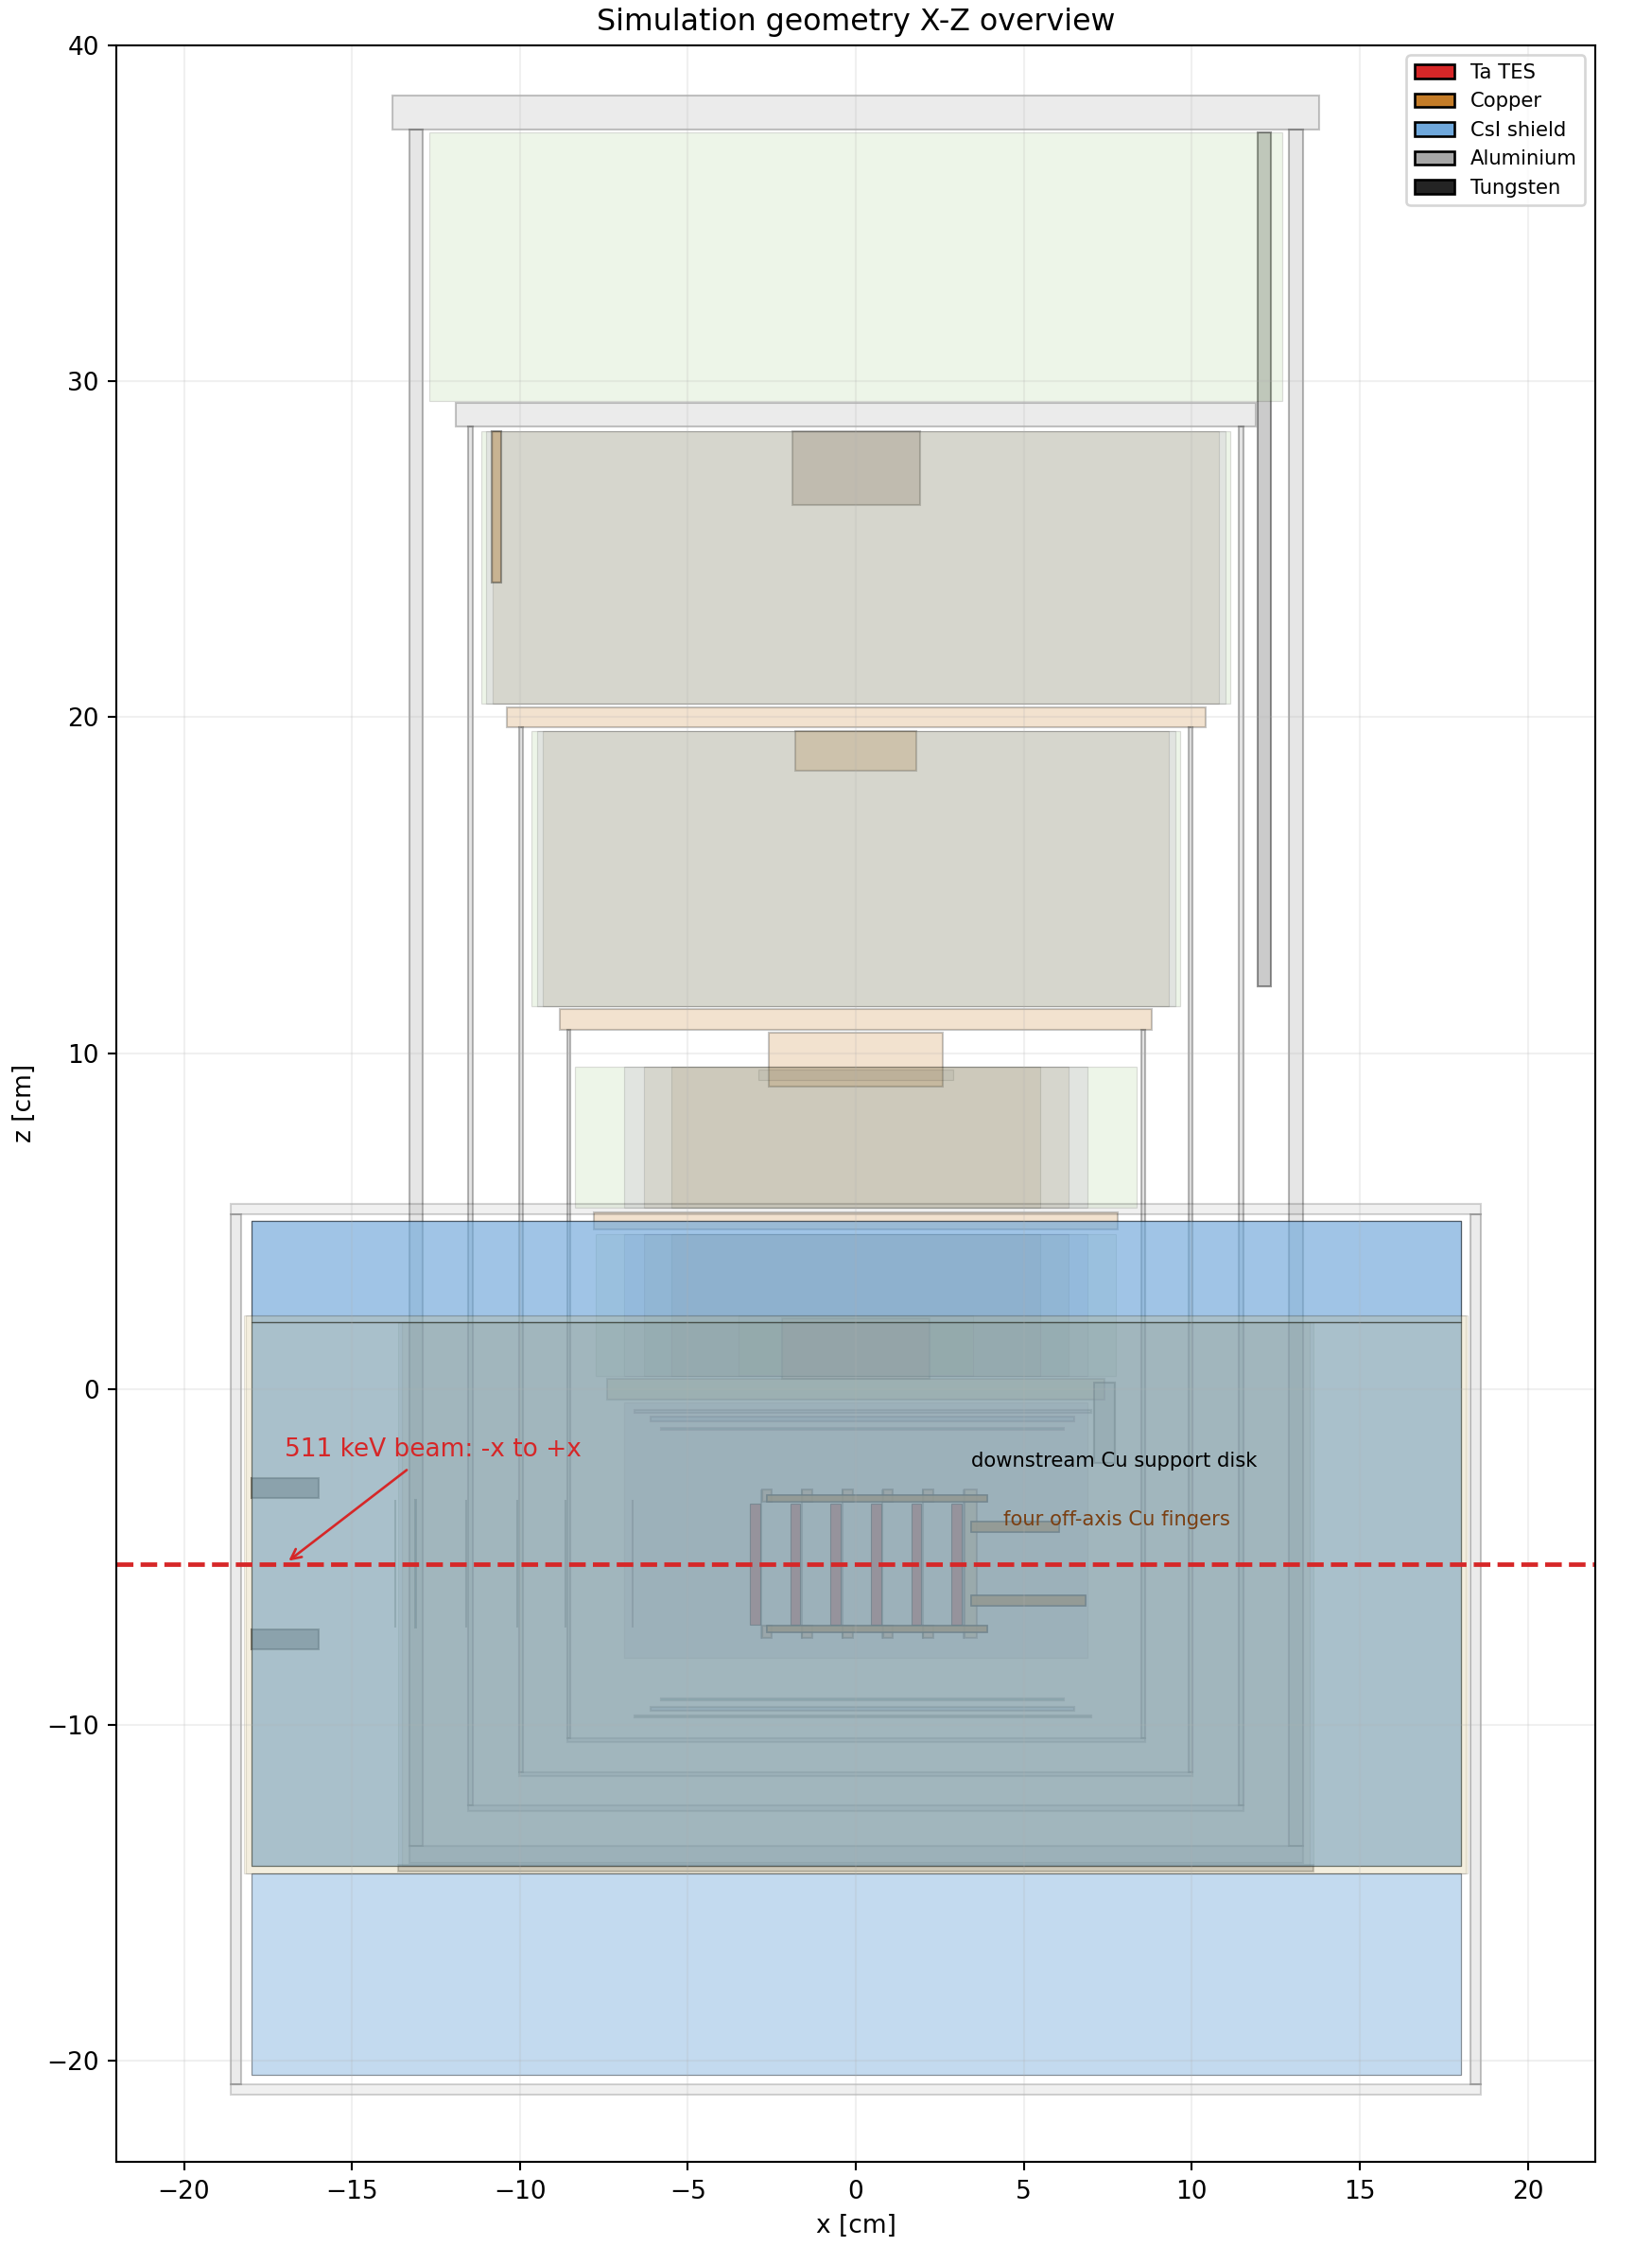
\includegraphics[width=0.62\linewidth]{paper_source_figure_table/fig_mass_model_xz_overview.png}

\vspace{0.6ex}
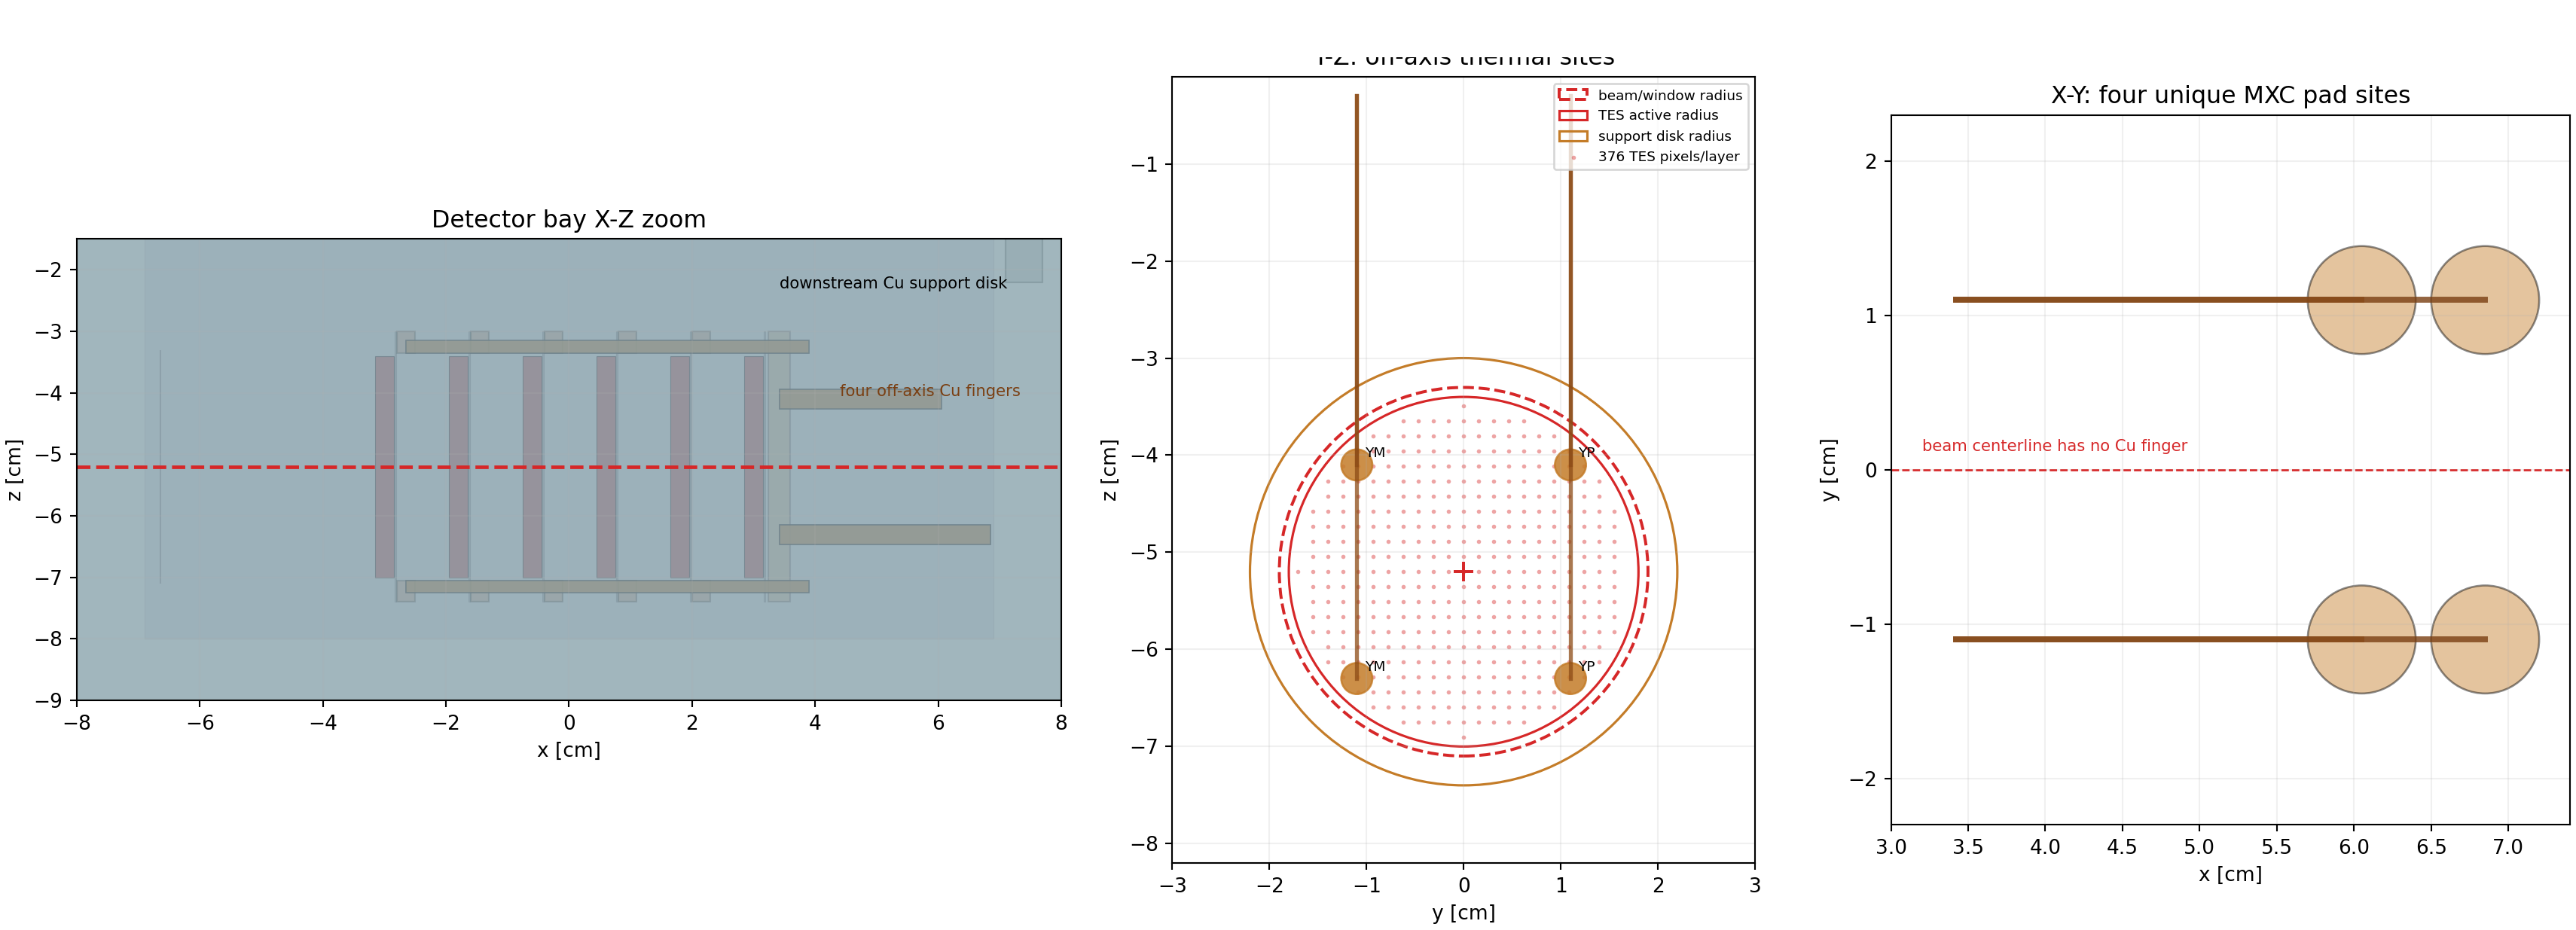
\includegraphics[width=0.88\linewidth]{paper_source_figure_table/fig_mass_model_detector_bay_detail.png}
\caption{Two-dimensional views of the baseline detector/cryostat proxy mass model. Top: full X--Z overview of the DR tower, detector bay, active shield, and side-entry 511 keV beam path. Bottom: detector-bay detail showing the TES absorber stack, open central beam region, and off-axis Cu thermal links. These are simulation schematics; circular x-axis parts and side apertures are represented by MEGAlib-compatible proxy shapes rather than final CAD solids.}
\label{fig:mass_model}
\end{figure}

\begin{table}[t]
\centering
\caption{Key detector and analysis parameters used for the primary exact-position chain.}
\label{tab:geometry}
\begin{tabular}{p{0.36\linewidth}p{0.56\linewidth}}
\toprule
Parameter & Value or policy \\
\midrule
Detector concept & TES microcalorimeter focal plane \\
TES pixel copies & $6\times376=2256$ \\
TES absorber proxy & Ta pixels, $1.5\times1.5\times3.0\,\mathrm{mm^3}$ each \\
TES energy-response proxy & Gaussian $\sigma=0.14\keV$ in the detector map \\
Detector efficiency & Geant4 transport plus downstream selected-rate normalization; no standalone scalar efficiency is imposed here \\
Active shield & Segmented CsI, post-processing veto \\
CsI veto threshold & $50\keV$ summed shield energy \\
Entrance-window stack & staged Al foils plus $150\,\mu\mathrm{m}$ Be side window \\
Passive shielding/collimation & Cu/W proxy liners, W bottom plate, and 2 cm W side sleeve \\
DR/service proxies & MXC/CP/still/4 K/60 K/300 K stage order plus local structural, cabling, and readout service-mass proxies \\
Pointing & Local side window tilted $45^\circ$ upward \\
Detector trigger/veto definition & Common detector-level post-processing selection \\
Coincidence window & $1\,\mu\mathrm{s}$ \\
Line window $\wii$ & $510.58$--$511.42\keV$ \\
Reference point-source flux $\fzero$ & $10^{-4}\cms$ \\
\bottomrule
\end{tabular}
\end{table}

\clearpage

\section{Laue optics and detector-coupled signal replay}
\label{sec:optics}

The signal model follows the standard Laue-lens approach in which mosaic crystals diffract incident gamma rays in transmission and concentrate them onto a small focal detector \cite{Barriere2009Laue,Barriere2011LauePrototype}. This is the same optical principle adopted in earlier focused gamma-ray telescope studies, where detector response must be evaluated together with the focused phase space rather than from lens effective area alone \cite{Weidenspointner2006MAX}. For the present 511 keV TES concept \cite{Shirazi2023}, the baseline optical configuration is a single-energy Ge(111) Laue ring with focal length $10\,\mathrm{m}$, 25 square tiles of 18 mm side length, 30 arcsec mosaic FWHM, and active Ge mass $0.44063\,\mathrm{kg}$. External XOP/CRYSTAL rocking-curve maps \cite{SanchezDelRio2011XOP} set the Ge(111) diffraction probability and angular response. The effective-area normalization is the ring geometric area multiplied by the simulated fraction of diffracted photons that emerge through the detector entrance aperture, giving $\aeff(511\keV)=20.08476\,\mathrm{cm^2}$.

The optical simulation is used as a source generator rather than as a standalone effective-area calculation. During transport, gamma rays that cross the nominal focal plane are recorded with their energy, position, direction, and production history. Only tracked diffracted photons that fall within the Be entrance-window aperture are passed downstream; analytic spot projections are retained only as diagnostics. This preserves the attenuation and scattering that occur while the diffracted photon exits the Ge crystal.

\begin{figure}[t]
\centering
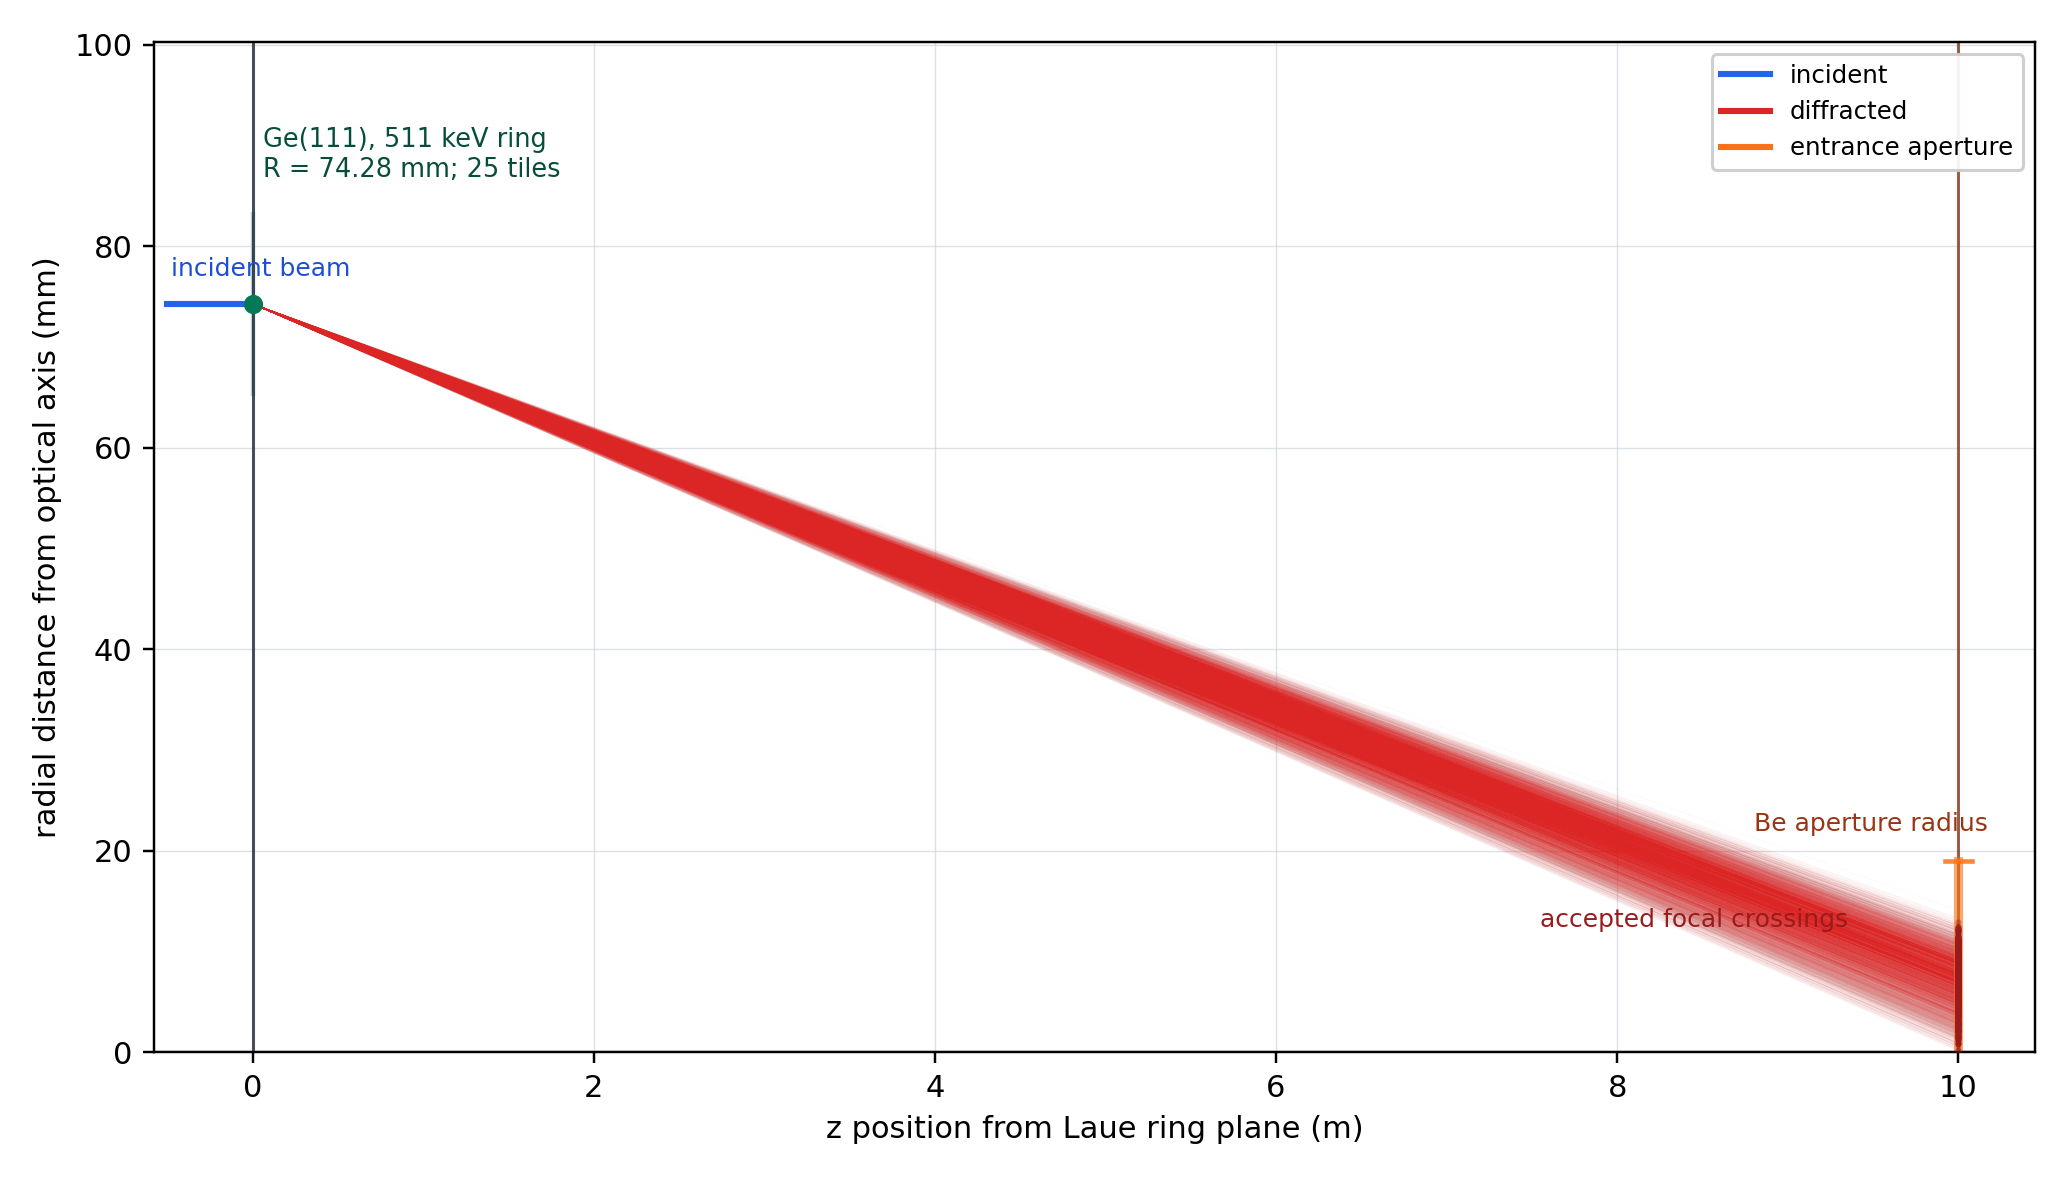
\includegraphics[width=0.96\linewidth]{paper_source_figure_table/fig_optics_laue_transport_schematic.png}
\caption{Data-constrained radial--$z$ visualization of the baseline 511 keV Laue signal source. The Laue plane, Ge(111) ring radius and tile footprint, $10\,\mathrm{m}$ focal distance, and Be entrance-aperture radius are read from the current optical configuration. The diffracted fan terminates on tracked focal-plane crossings that satisfy the entrance-aperture gate. The plot collapses the azimuthal tile layout and is used only to visualize the transport-backed detector input.}
\label{fig:optics_transport_schematic}
\end{figure}

\begin{figure}[t]
\centering
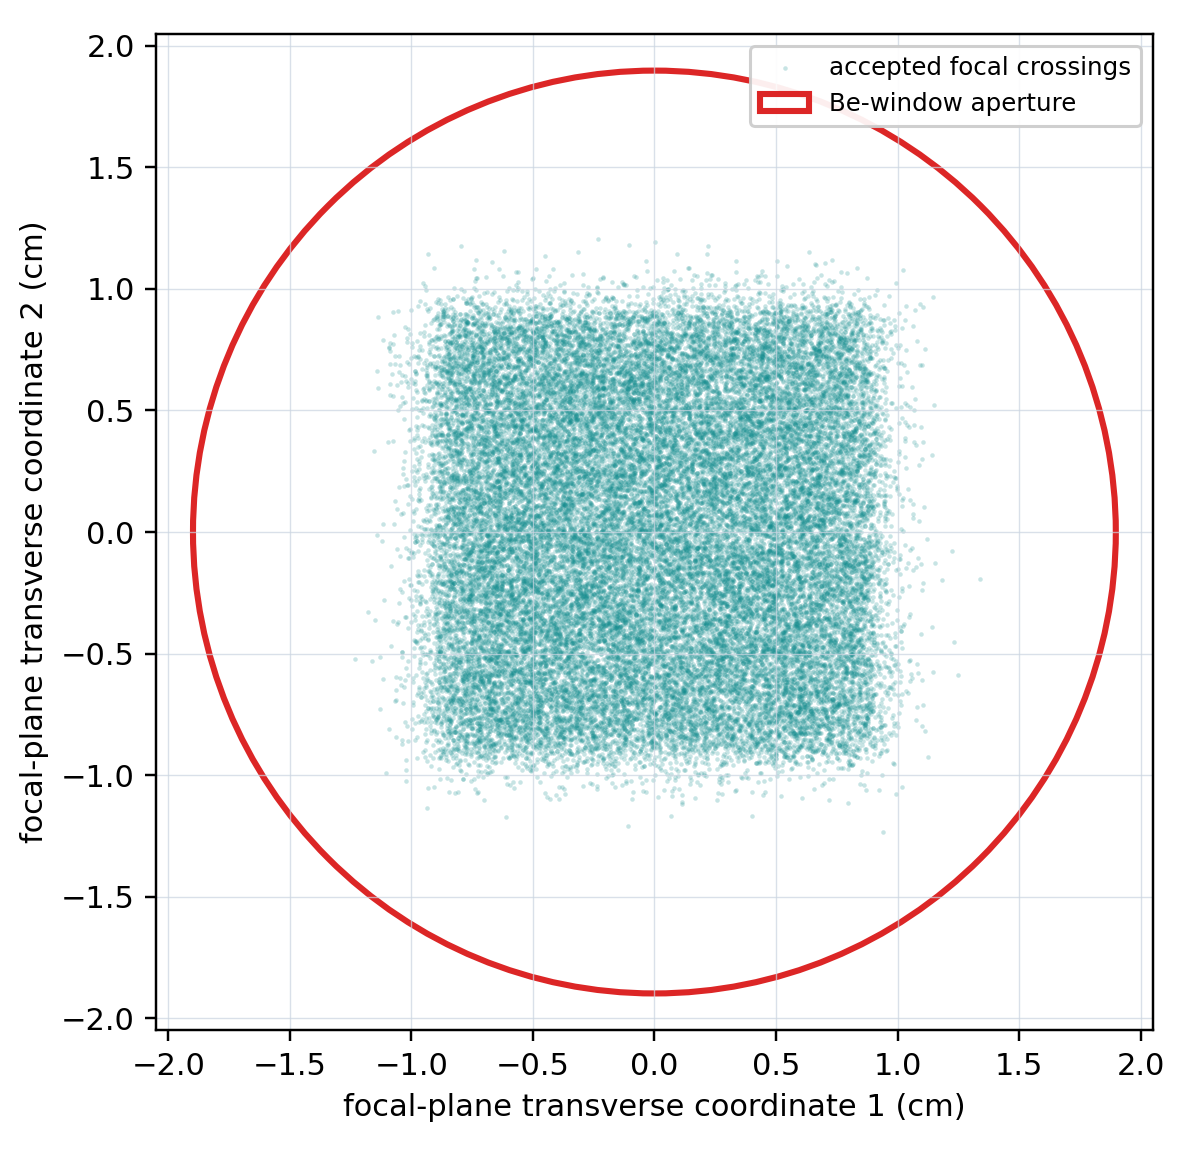
\includegraphics[width=0.58\linewidth]{paper_source_figure_table/fig_optics_focal_crossings_xy.png}
\caption{Tracked transverse focal-plane positions accepted by the Be entrance aperture and used for downstream detector replay. The red circle marks the Be-window aperture. This is the transported optical phase-space distribution at the detector input plane, not an analytic focal-spot projection.}
\label{fig:optics_focal_spot}
\end{figure}

Figures~\ref{fig:optics_transport_schematic} and \ref{fig:optics_focal_spot} show the two levels of the optics-detector coupling: the radial optical constraint from the configured Laue ring to the focal plane, and the transverse distribution injected into the detector model. The accepted focal-plane particles are transformed into the local side-entry detector coordinate system and replayed through the detector/cryostat mass model. This keeps the simulated entrance position and direction distribution, rather than replacing the optical calculation with an analytic focal spot. The focal-plane crossing table used here is therefore a transported optical-signal input: it records gamma rays from the 511 keV source simulation that cross the focal plane, not particles produced by atmospheric or cosmic-ray interactions in the upstream lens hardware.

An auxiliary upstream-hardware closure branch was run to test that this boundary can be treated by the same Geant4/MEGAlib background machinery when needed. The branch places an equal-volume and equal-mass Ge proxy for the active Laue crystals at the 10 m upstream lens position. The proxy corresponds to 25 square Ge tiles of 18 mm side length and 10.218801 mm thickness, giving active Ge volume $82.7723\,\mathrm{cm^3}$ and mass $0.4406\,\mathrm{kg}$. The atmospheric far-field source surface is not inherited from the local 60 cm detector source sphere. Instead, it is derived from the combined detector-plus-lens enclosing radius: the 10 m lens center plus the active-crystal volume bound gives $1008.8\,\mathrm{cm}$, and the transport source surface is rounded upward to a radius of $1060\,\mathrm{cm}$ inside a $2500\,\mathrm{cm}$ world half-size. After low-statistics interface tests, production prompt and activation-production transports were run for the proxy with the same eight EXPACS/PARMA particle families ($\gamma$, $n$, $e^\pm$, $p$, $\alpha$, and $\mu^\pm$) used in the detector-background chain. These runs close the full-particle transport and isotope-production boundary for the upstream mass proxy.

The delayed component from the active-Ge proxy was then isolated from the combined isotope-production records and converted into a decay source at the recorded production positions. It contains two day-15 radioisotope records, $^{70}$Ga and $^{73}$Ga, with total activity $0.425674\,\mathrm{Bq}$. A 20,000-trigger delayed transport through the same detector geometry and detector-level selection produced no selected $\wii$ events; the corresponding direct selected rate is zero, with a 95\% zero-count upper rate of $1.25\times10^{-4}\cps$. This upper limit is about $0.20\%$ of the primary exact-position $\wii$ background rate, $0.0629804\cps$, so it does not change the quoted hard-window sensitivity at the current precision. The prompt self-background from upstream hardware is still not folded into the primary budget because the combined prompt simulation also contains the ordinary detector/cryostat atmospheric prompt background and needs provenance isolation or subtraction. Explicit lens-tile supports remain a separate design-level systematic.

For the focused point-source response, $\fzero=10^{-4}\cms$ denotes the reference incident 511 keV photon flux. The quoted hard-window signal response, $0.00118117\cps$, is the selected $\wii$ signal rate at that flux after detector transport and detector-level event selection. The source-flux response is the corresponding linear coefficient, $S_{\wii}/\fzero=11.8117\,\mathrm{s^{-1}}/(\mathrm{ph\,cm^{-2}\,s^{-1}})$.

\section{Prompt atmospheric and delayed-activation source model}
\label{sec:background}

\subsection{Prompt atmospheric source}
\label{subsec:prompt_source}

The background source model is separated into prompt atmospheric transport and delayed activation so that source generation does not absorb assumptions that belong to detector selection. The prompt atmospheric field is derived from EXPACS/PARMA. PARMA3.0 is an analytical model parameterized from PHITS atmospheric-shower calculations and benchmarked for terrestrial cosmic-ray fields, and EXPACS is its public tabulation/software interface \cite{Sato2015EXPACS}. PHITS supplies the underlying particle-transport calculation for cosmic-ray interactions in the atmosphere: primary cosmic rays interact with air nuclei, secondary hadrons, leptons, photons, and neutrons are transported through the atmospheric column, and the resulting particle fluences are parameterized by altitude, geomagnetic cutoff, solar modulation, energy, and direction. In this work EXPACS/PARMA provides the differential incident particle flux as a function of particle species, kinetic energy, zenith angle, geographic position, altitude, geomagnetic cutoff rigidity, and solar modulation. It is used only to construct the external radiation fields; detector response, vetoing, topology selection, and mission-time counting are applied later. The reference source cards use latitude $34^\circ$, longitude $100^\circ$, altitude $38\,\mathrm{km}$, vertical cutoff rigidity $R_c=11.6\,\mathrm{GV}$, and the 2025-08-31 solar condition corresponding to $W=118.3$.

The prompt source includes photons, neutrons, electrons, positrons, protons, alpha particles, negative muons, and positive muons. For each particle family, the EXPACS/PARMA differential spectrum is converted into a MEGAlib far-field area source over the full zenith range $\theta=0^\circ$--$180^\circ$ and full azimuth range $\phi=0^\circ$--$360^\circ$. The zenith dependence is represented by 20 differential equal-$\mu$ angular bins, where $\mu=\cos\theta$ and each bin subtends $\Delta\Omega=0.6283185307\,\mathrm{sr}$. The first ten bins cover down-going particles ($0^\circ\leq\theta\leq90^\circ$), and the last ten bins cover up-going or albedo-like particles ($90^\circ\leq\theta\leq180^\circ$). Both hemispheres are retained in both the prompt transport and the activation-production transport, so upward albedo particles are not discarded at source construction.

\begin{figure}[t]
\centering
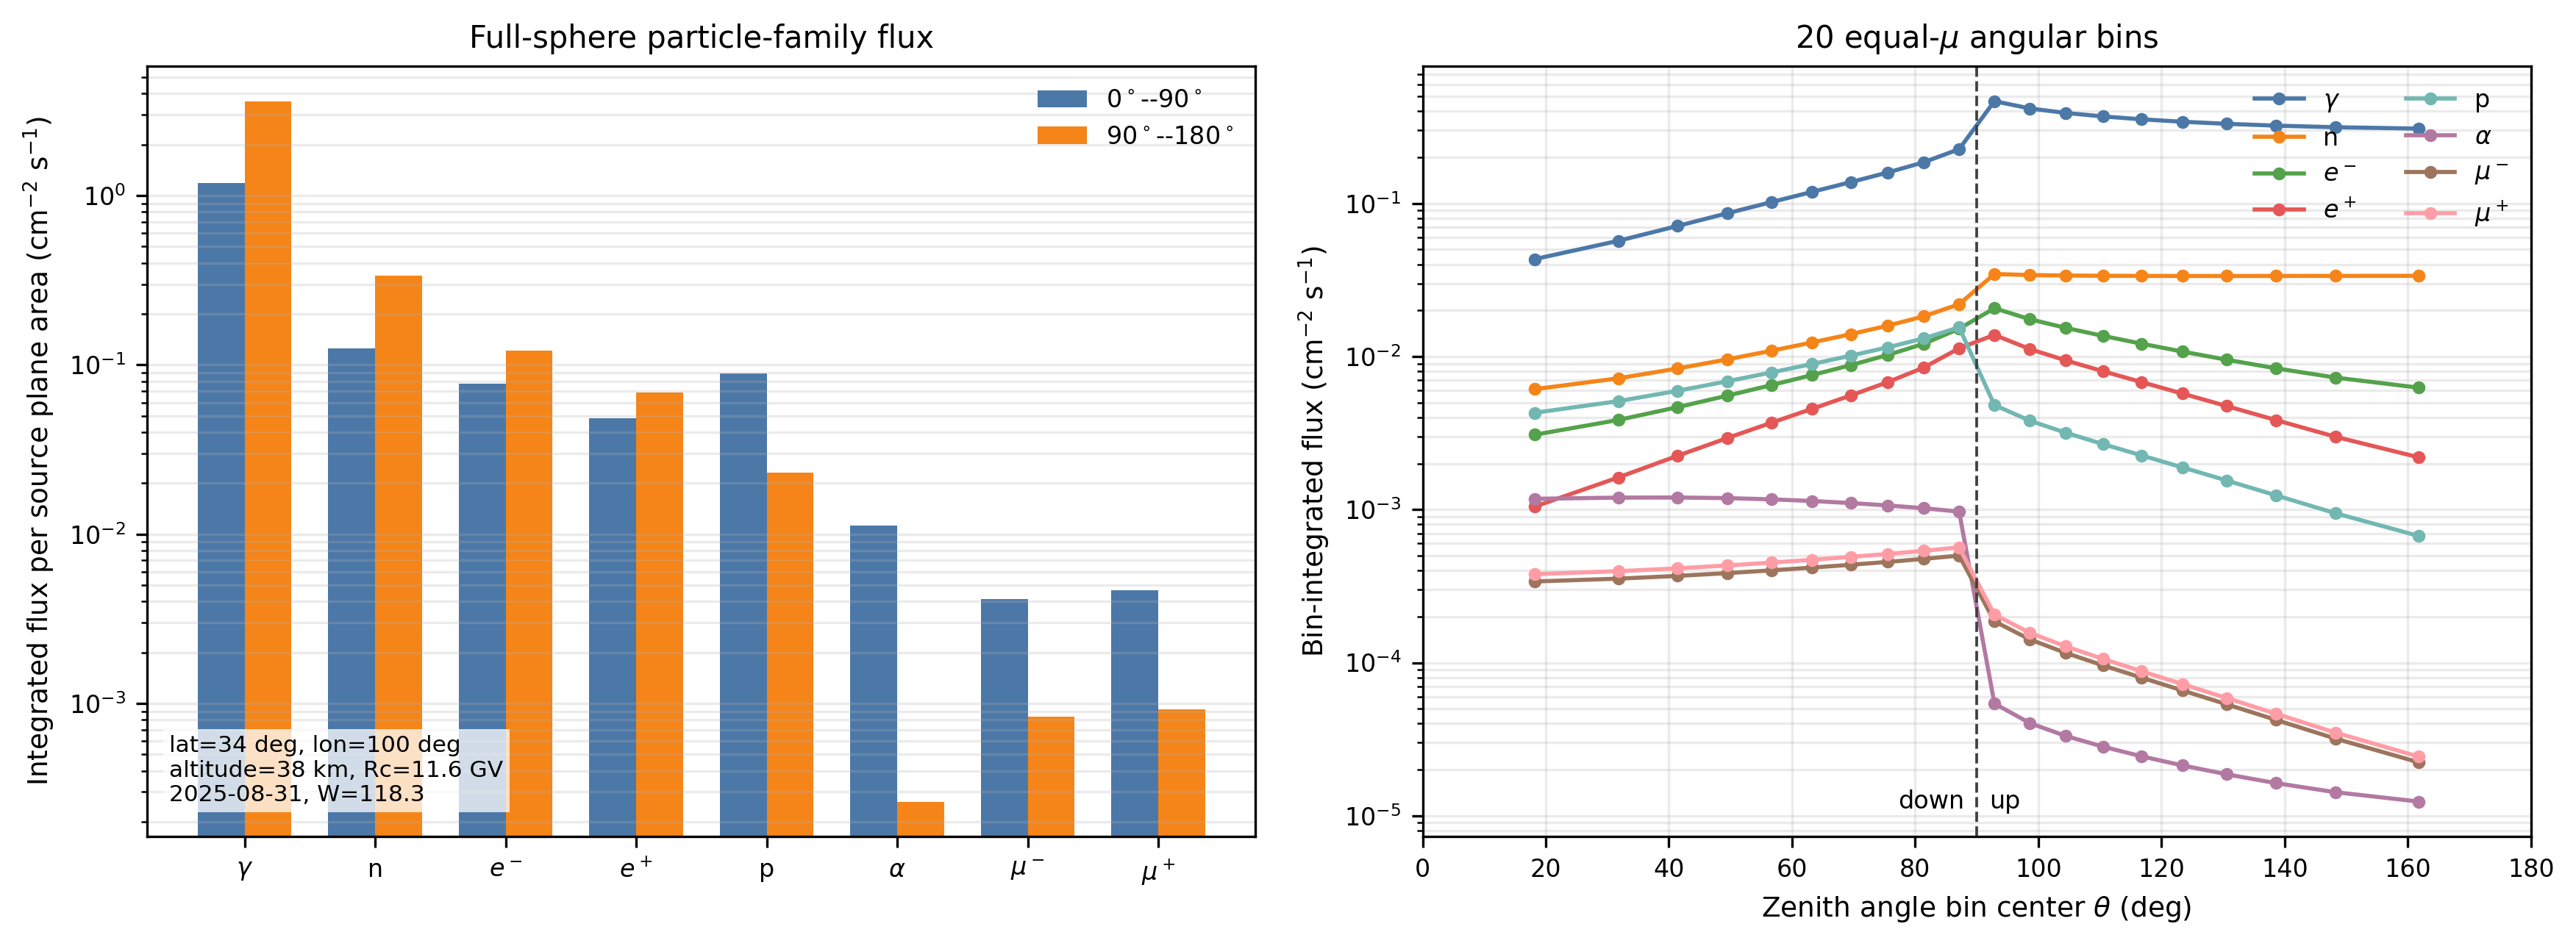
\includegraphics[width=\linewidth]{paper_source_figure_table/fig_expacs_fullsphere_flux.png}
\caption{EXPACS/PARMA full-sphere atmospheric flux field used to generate the prompt and activation-production source cards. Left: energy- and solid-angle-integrated fluxes for the eight transported particle families, separated into down-going and up-going hemispheres. Right: bin-integrated flux in the 20 equal-$\mu$ differential zenith bins used by the MEGAlib far-field source. The plot is generated from the source-card inputs for latitude $34^\circ$, longitude $100^\circ$, altitude $38\,\mathrm{km}$, $R_c=11.6\,\mathrm{GV}$, and $W=118.3$.}
\label{fig:expacs_fullsphere_flux}
\end{figure}

Figure~\ref{fig:expacs_fullsphere_flux} shows the resulting full-sphere flux field. The integrated source-plane fluxes are $4.79966$, $0.462239$, $0.199002$, $0.116981$, $0.112301$, $0.0114871$, $0.00496893$, and $0.00557001\,\mathrm{cm^{-2}\,s^{-1}}$ for $\gamma$, $n$, $e^-$, $e^+$, $p$, $\alpha$, $\mu^-$, and $\mu^+$, respectively. The non-photon components therefore carry about $0.913\,\mathrm{cm^{-2}\,s^{-1}}$, or 16\% of the total full-sphere source-plane flux. To keep their detector and activation statistics from being limited by strict flux-proportional event counts, the non-photon particle families are generated with replicated Monte Carlo samples and then de-weighted in the rate normalization. In the full-statistics prompt chain, the photon stream is split into 12 jobs, while each non-photon family is run in eight independent replicas. These particles are transported through the detector/cryostat mass model with Geant4/MEGAlib \cite{Agostinelli2003,Zoglauer2006}. The prompt run and the activation-production run each generated 25,210,216 incident primary particles. The prompt input is split into 68 transported products, and each particle species is normalized with its own transported exposure using
\begin{equation}
  r_{\mathrm{event},j}=\left(\sum_i \mathcal{T}_{ij}\right)^{-1},
\end{equation}
where $\mathcal{T}_{ij}$ is the transported exposure of split product $i$ for particle species $j$. This per-species normalization is required because photon and non-photon atmospheric streams have different splitting and exposure structures. The prompt normalization audit enforces $r_{\mathrm{event},j}\sum_i\mathcal{T}_{ij}=1$ for each particle species, so over-sampling changes the Monte Carlo variance but not the expected physical rate.

\subsection{Delayed activation source}
\label{subsec:delayed_source}

The activation-production stream is not counted as an immediate detector background. Instead, it records the isotope, material volume, and production position of radioactive products. These records are converted into a fixed day-15 radioactive population using production--decay buildup equations and ground-state half-life corrections audited against NUBASE2020 \cite{Kondev2021NUBASE}. For isotope $k$,
\begin{equation}
  A_k(t_{\mathrm{flight}}) = R_k\left[1-\exp\left(-\lambda_k t_{\mathrm{flight}}\right)\right],
  \qquad \lambda_k = \frac{\ln 2}{t_{1/2,k}},
\end{equation}
where $R_k$ is the production rate inferred from the activation-production transport and $t_{\mathrm{flight}}=15\,\mathrm{d}$ for the reference day-15 state. The resulting fixed delayed activity used by the baseline chain is $85.636696\,\mathrm{Bq}$.

The position information is not obtained from the aggregate isotope store alone. The standard isotope store records the volume name and isotope count, while the exact-position chain also uses a custom hook in the Geant4/MEGAlib stepping-action layer. At the same point where an isotope is stored during activation buildup, the hook writes a production-position record containing the logical volume, pre-step position $(x,y,z)$, isotope identifier $1000Z+A$, excitation energy, time, process, and track ancestry metadata. The fixed day-15 isotope population is then joined to these records by volume, isotope, and excitation state. This gives the delayed source access to the true simulated production coordinates rather than only to volume-integrated activities.

\begin{figure}[t]
\centering
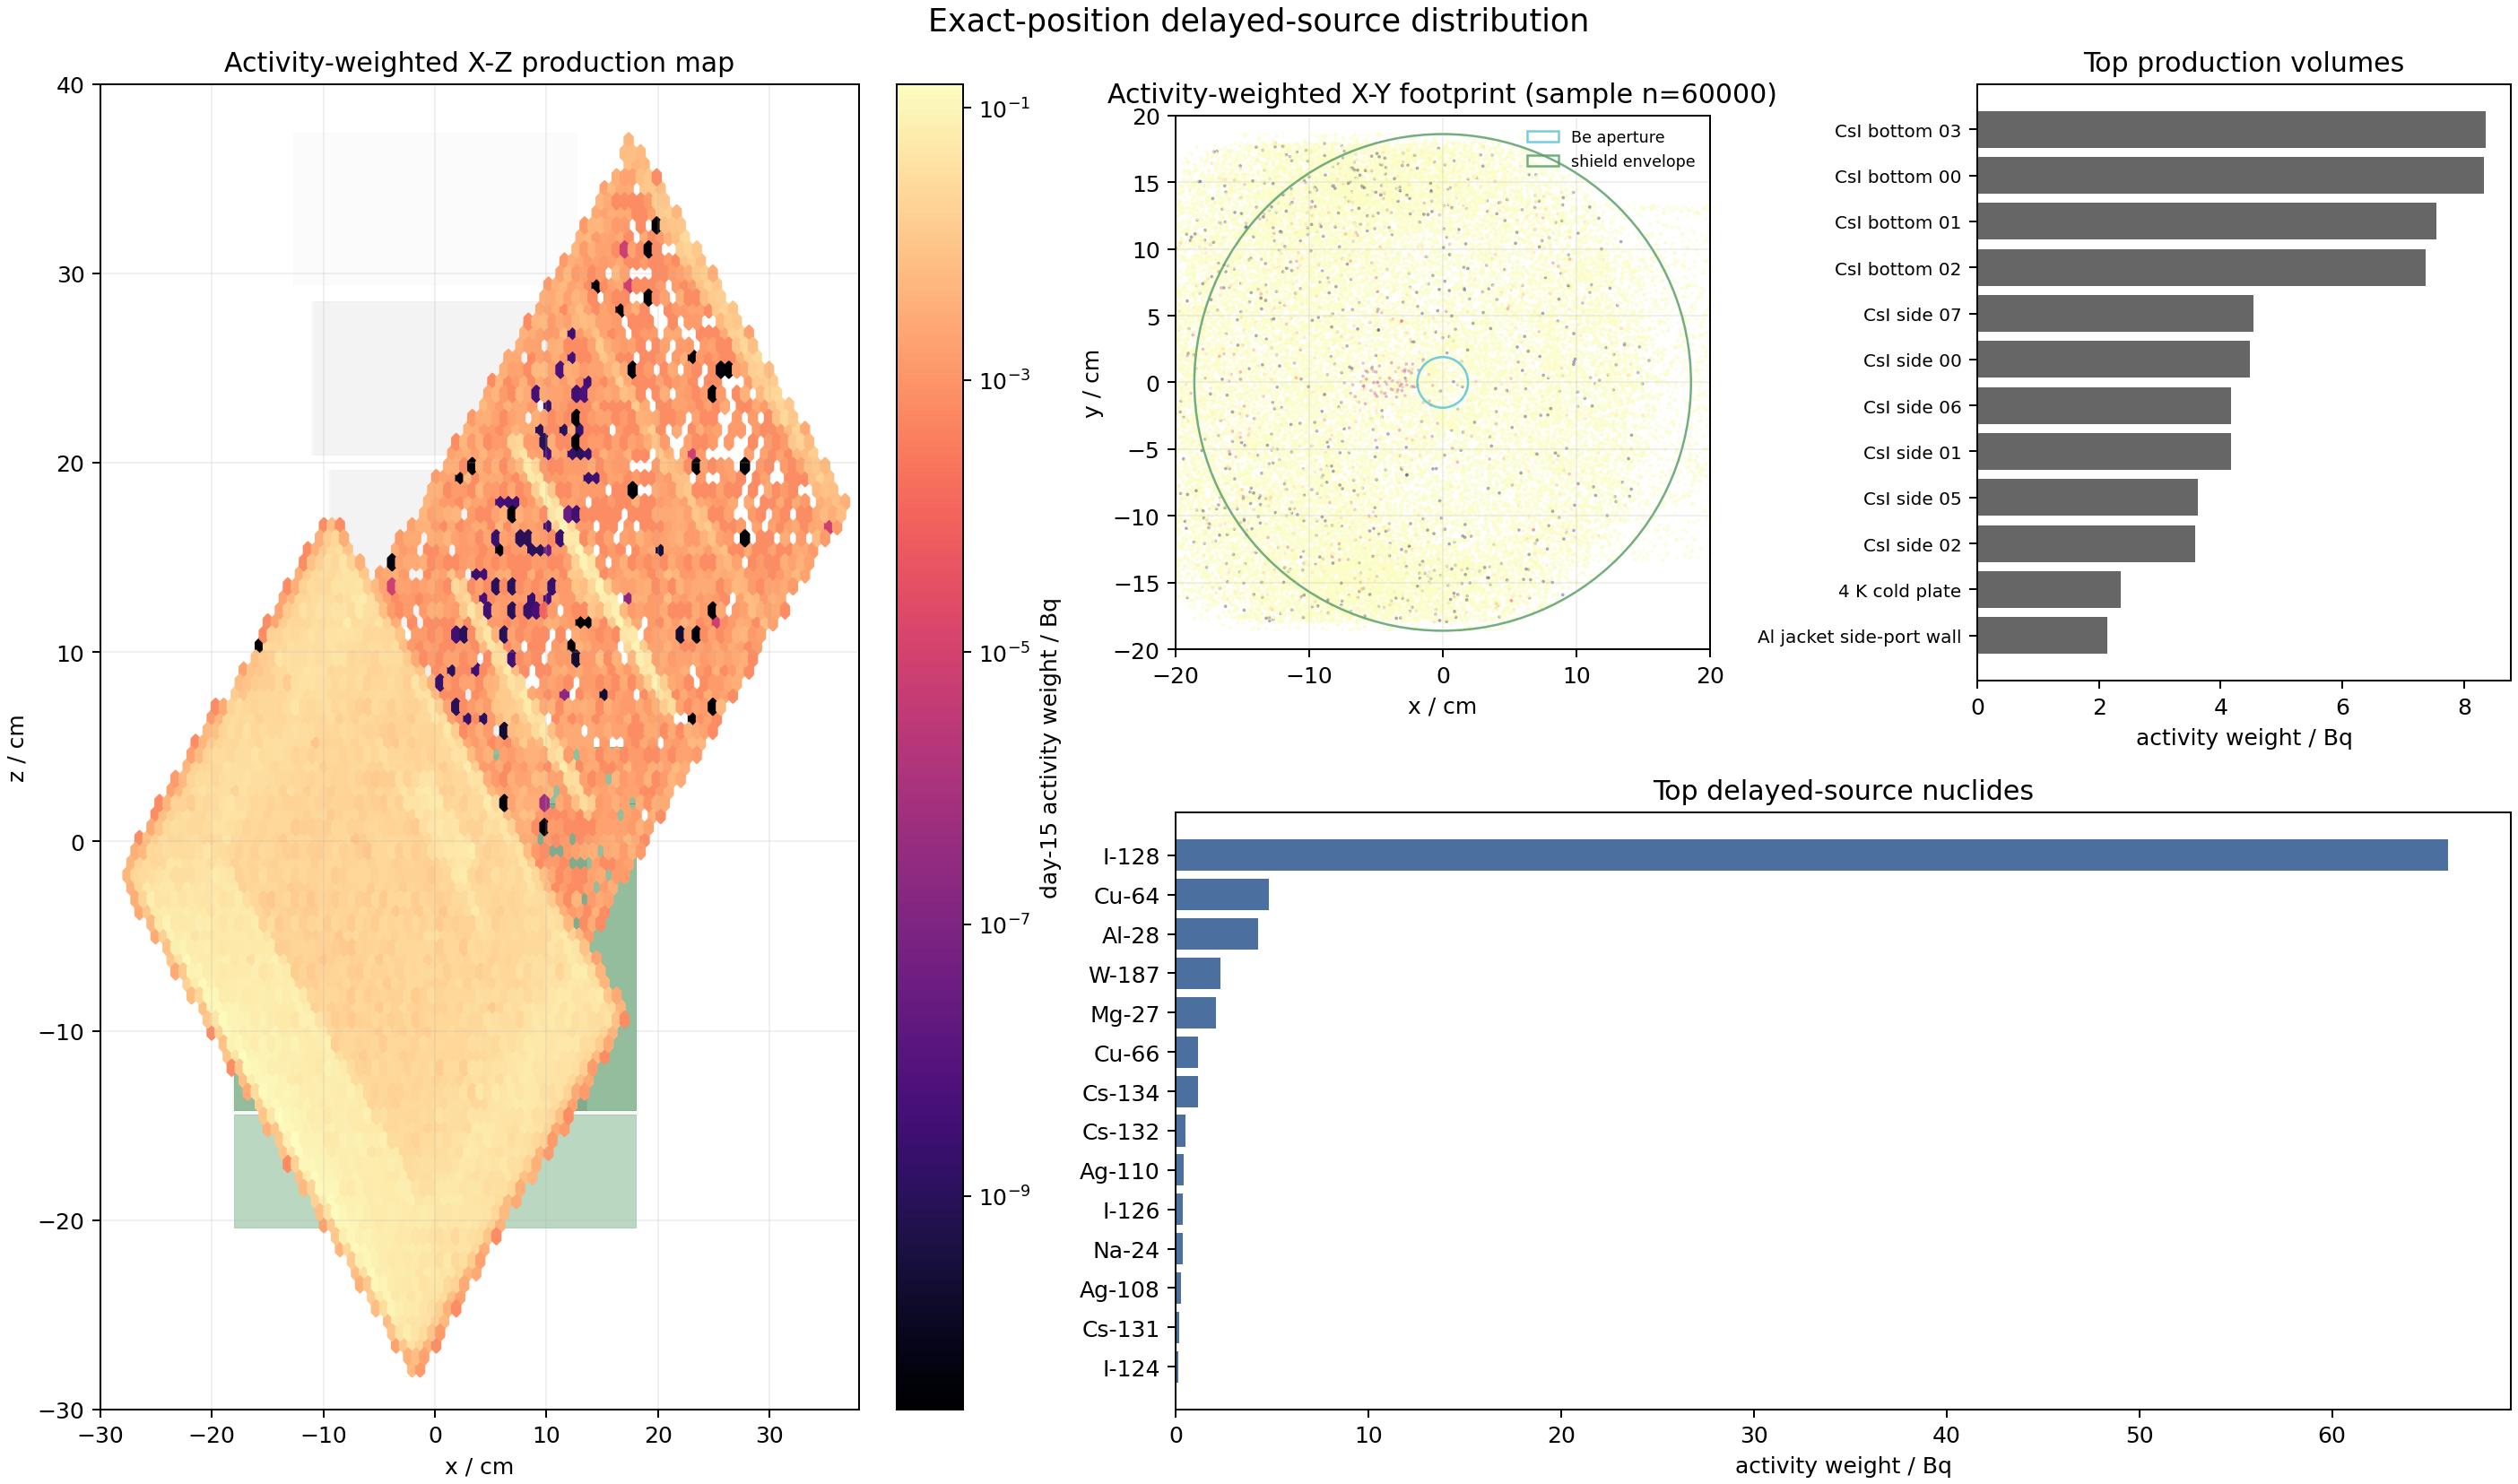
\includegraphics[width=\linewidth]{paper_source_figure_table/fig_delayed_exactpos_rpip_distribution.png}
\caption{Exact-position delayed-source support constructed from true radioactive-isotope production positions. Left: activity-weighted X--Z map of the recorded production positions overlaid on the detector/cryostat proxy geometry. Top middle: activity-weighted X--Y footprint sampled from the same distribution, with the Be aperture and shield envelope shown for scale. Right and bottom: leading production volumes and nuclides after fixed day-15 activity weighting. The figure is built from 253,770 eligible weighted production-position rows, whose weights sum to $85.636696\,\mathrm{Bq}$.}
\label{fig:delayed_exactpos_distribution}
\end{figure}

Figure~\ref{fig:delayed_exactpos_distribution} shows the resulting delayed-source position distribution. The current exact-position table parses 68 activation-production files, finds 259,808 radioactive-production position records, and writes 253,770 eligible weighted rows after matching to the fixed day-15 activity population. The activity-weighted distribution is dominated by CsI shield activation and by $^{128}$I, with smaller contributions from Cu, Al, W, Mg, and Cs isotopes. The figure is a source-construction diagnostic, not a detector-count map; detector response is applied only after the delayed decays are transported through the common geometry and event selection.

The need for exact-position sampling is also testable from the same production table. Delayed decays are emitted locally, so the downstream attenuation, active-shield veto probability, and event topology depend on where the isotope was produced. Charged hadrons and muons have different energy-loss, stopping, and capture histories from neutrons, and therefore need not produce an exchangeable material or coordinate distribution. To quantify this, the weighted production rows were grouped by incident particle family and by material category. For two families $a$ and $b$, we compare the activity-normalized category distributions with
\begin{equation}
  D_{\mathrm{TV}}(a,b) =
  \frac{1}{2}\sum_c \left| f_{a,c} - f_{b,c} \right| ,
\end{equation}
where $f_{a,c}$ is the fraction of delayed activity from incident family $a$ produced in material category $c$.

\begin{figure}[t]
\centering
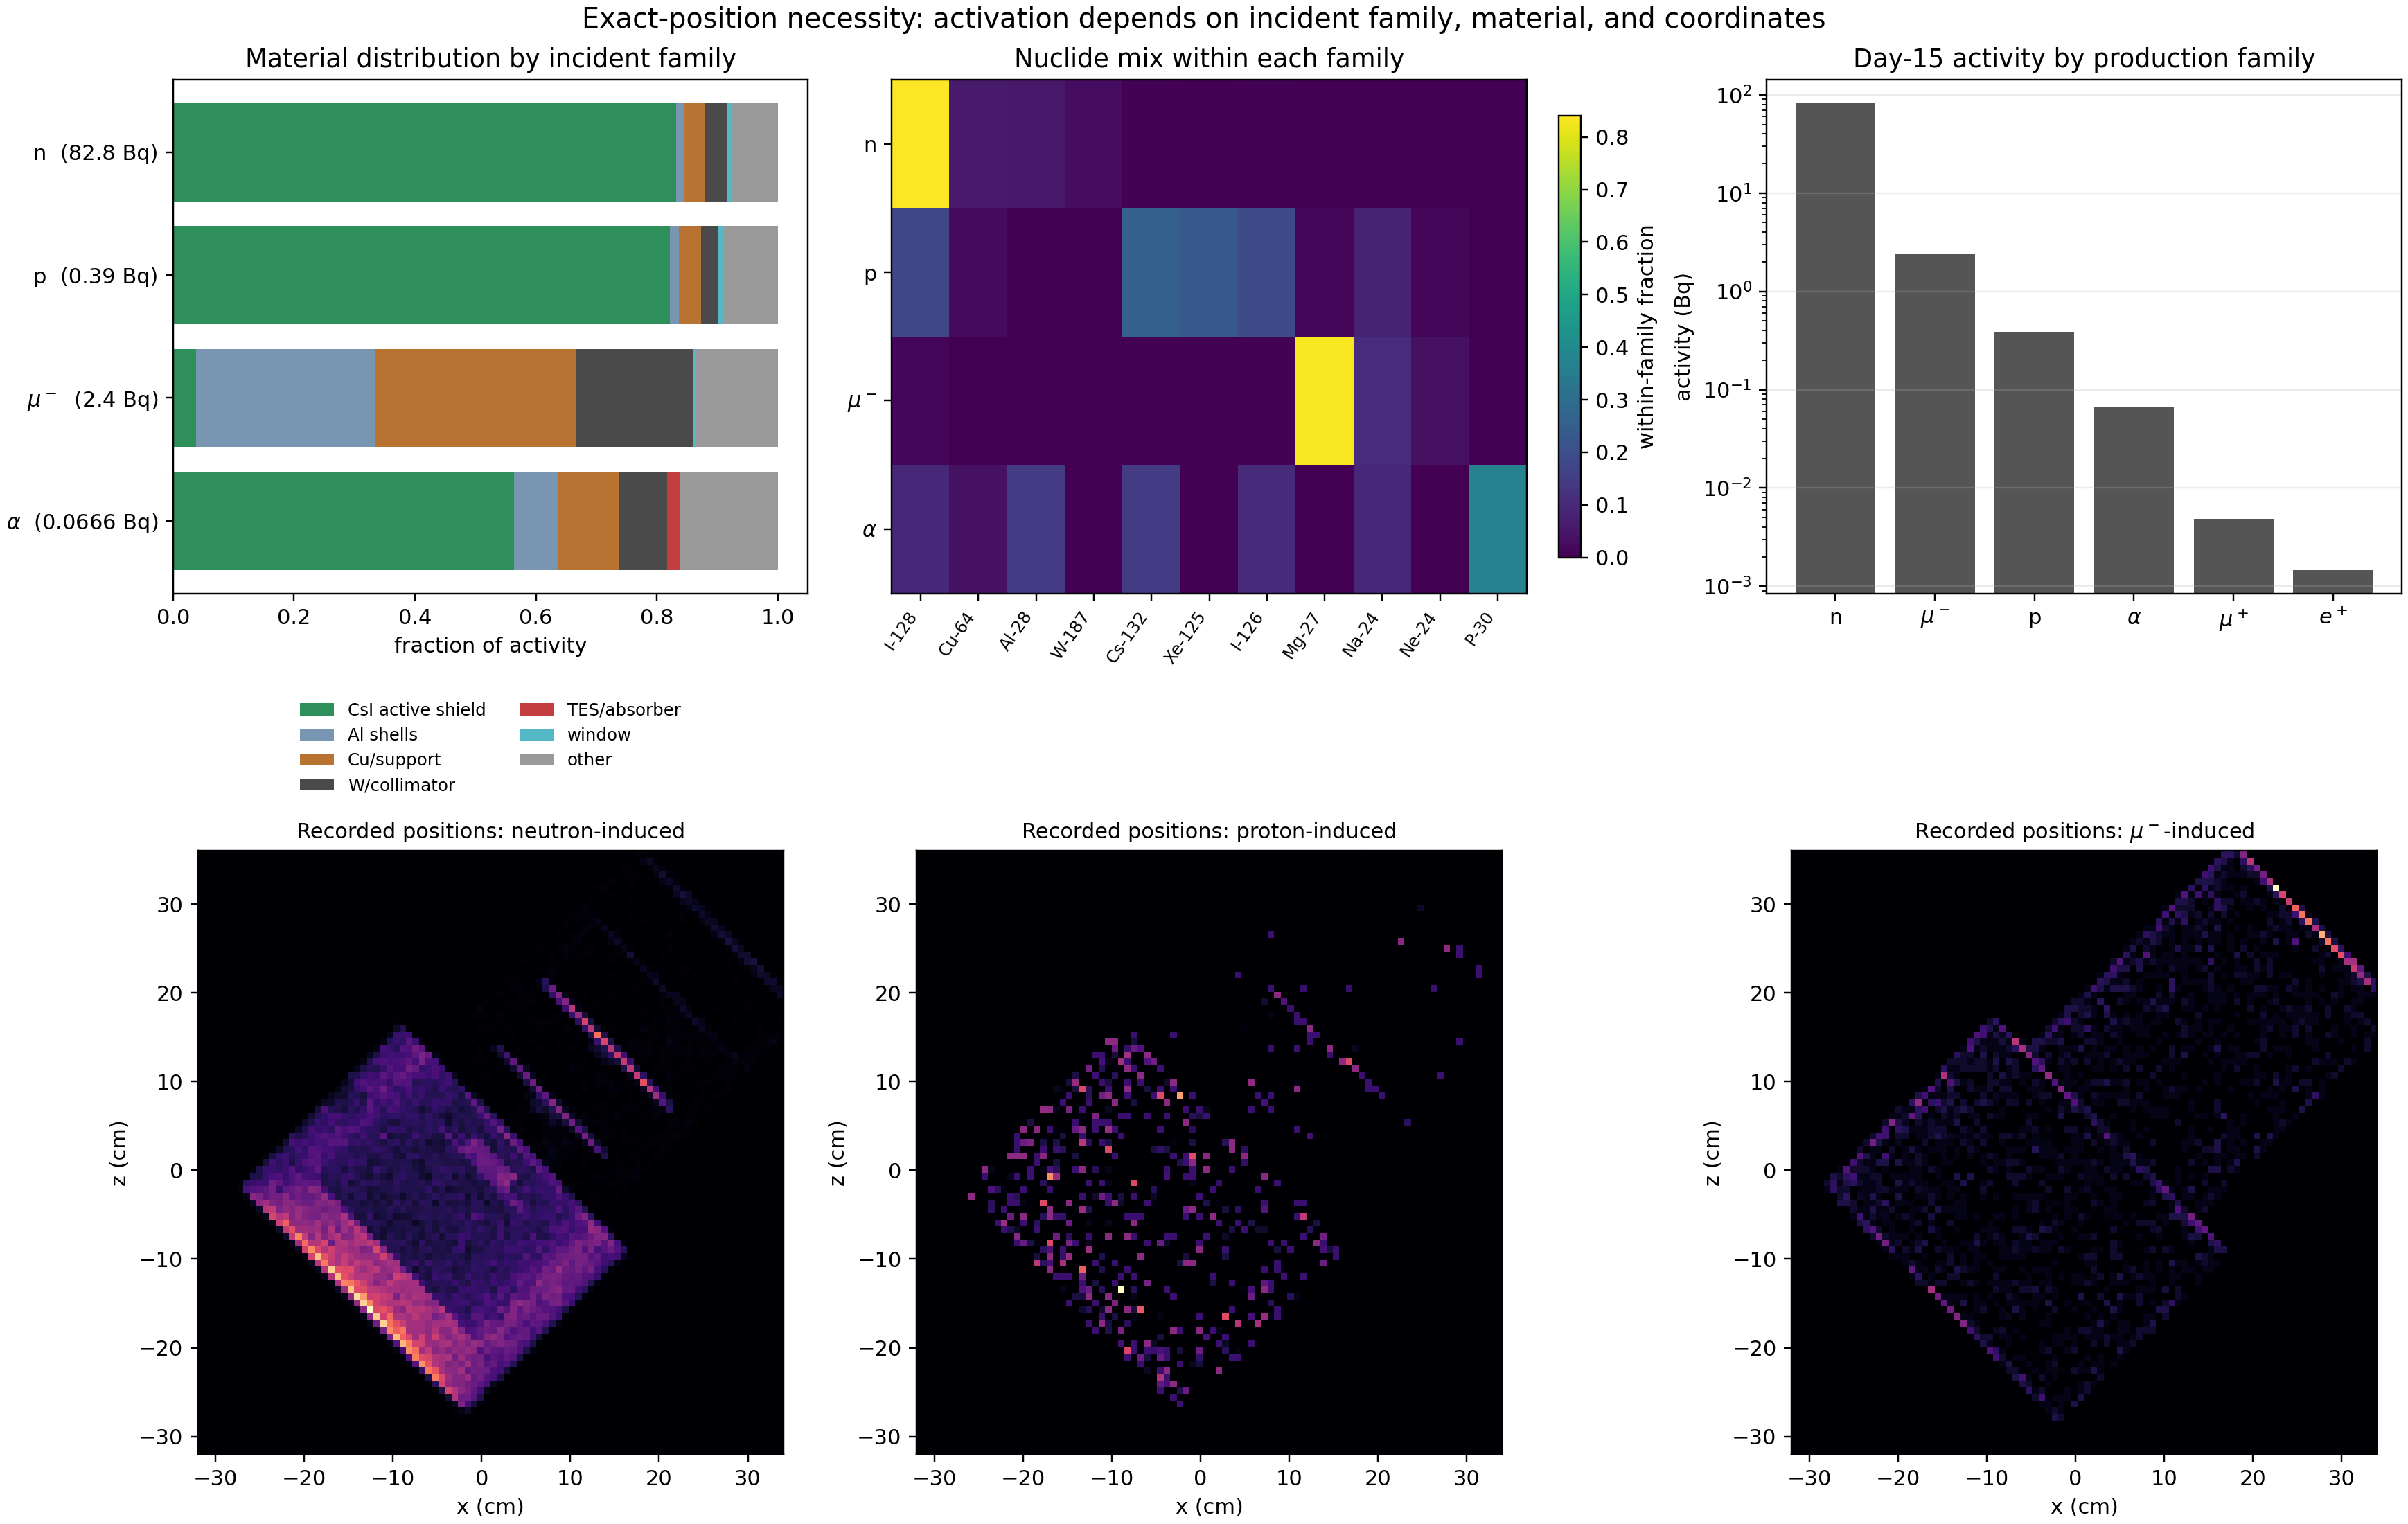
\includegraphics[width=\linewidth]{paper_source_figure_table/fig_exactpos_sampling_necessity.png}
\caption{Data-backed necessity test for exact-position delayed-source sampling. The upper panels compare the day-15 weighted production table by incident particle family: material fractions, nuclide mix, and total activity. The lower panels show the recorded X--Z production-position maps for neutron-, proton-, and $\mu^-$-induced products. The distributions are not exchangeable: neutron-induced activity is dominated by CsI and $^{128}$I, while $\mu^-$-induced activity is concentrated in Al/Cu/W service and shield material and is dominated by Mg/Na/Ne products.}
\label{fig:exactpos_sampling_necessity}
\end{figure}

Figure~\ref{fig:exactpos_sampling_necessity} gives the result of this test. In the fixed day-15 table, neutron-induced products contribute $82.769\,\mathrm{Bq}$, $\mu^-$-induced products contribute $2.405\,\mathrm{Bq}$, proton-induced products contribute $0.390\,\mathrm{Bq}$, and $\alpha$-induced products contribute $0.0666\,\mathrm{Bq}$. The neutron and proton categories are mostly produced in the CsI active shield, with CsI fractions of $83.2\%$ and $82.1\%$, respectively. The $\mu^-$ component is qualitatively different: only $3.78\%$ of its weighted activity is in CsI, while Al shells, Cu/support material, and W/collimator material account for $29.6\%$, $33.2\%$, and $19.4\%$. The corresponding material-distribution distances are $D_{\mathrm{TV}}(n,\mu^-)=0.798$ and $D_{\mathrm{TV}}(p,\mu^-)=0.787$. The coordinate distribution also shifts: the activity-weighted median $z$ coordinate is $-7.60\,\mathrm{cm}$ for neutron-induced products, $-3.31\,\mathrm{cm}$ for proton-induced products, and $+8.27\,\mathrm{cm}$ for $\mu^-$-induced products. The leading nuclides differ as well, with neutron-induced activity dominated by $^{128}$I, $\mu^-$-induced activity dominated by $^{27}$Mg, $^{24}$Na, and $^{24}$Ne, and proton-induced activity distributed among Cs, Xe, and I isotopes. A volume-integrated or axisymmetric radial source could preserve total activity, but it would remove these incident-family, material, nuclide, and coordinate correlations. The exact-position construction keeps them in the source distribution before detector transport.

The delayed-decay source is launched from sampled production positions rather than from an axisymmetric radial profile. Let rows $j$ in the weighted production table have activity weights $w_j$ with total activity $A=\sum_j w_j$. The exact-position approximation draws $M$ support locations with replacement using probabilities $p_j=w_j/A$, and assigns each support element flux $A/M$. The expected activity assigned to row $j$ is therefore
\begin{equation}
  \mathbb{E}\!\left[N_j\frac{A}{M}\right] = M p_j \frac{A}{M} = w_j ,
\end{equation}
so the estimator is activity preserving and unbiased for the weighted spatial distribution. Here $M$ denotes the number of equal-activity point-source support elements used to approximate the distribution; it is a sampling support size, not the number of physical isotope-production rows. The nominal paper-facing source uses $M=50000$ point-source support elements drawn from the 253,770 weighted rows, while the smaller $M=5000$ and $M=20000$ cases are retained as convergence checks. The support elements preserve the total fixed activity exactly at the source-definition level and are replayed through the same detector/cryostat geometry used for the prompt stream. The nominal delayed transport used $10^6$ triggers and stored $10^6$ events, with Cosima live time $11545.456287\,\mathrm{s}$. This live time is a transport record for the generated decay sequence and is not used as the physical balloon exposure.

\begin{table}[t]
\centering
\caption{Background-source layers used by the baseline detector-coupled chain. The table defines the source construction only; vetoes, topology cuts, and the hard line window are applied later in Section~\ref{sec:selection}.}
\label{tab:background_source_model}
\begin{tabular}{p{0.22\linewidth}p{0.34\linewidth}p{0.34\linewidth}}
\hline
Layer & Physical role & Baseline implementation \\
\hline
Prompt atmospheric transport & Direct detector hits from atmospheric secondaries & EXPACS/PARMA full-sphere source cards at $34^\circ$ latitude, $100^\circ$ longitude, $38\,\mathrm{km}$ altitude, $R_c=11.6\,\mathrm{GV}$, and $W=118.3$; $\gamma$, $n$, $e^\pm$, $p$, $\alpha$, and $\mu^\pm$ over 20 equal-$\mu$ differential zenith bins including both down-going and up-going hemispheres; 25,210,216 generated primaries. \\
Activation production & Radioisotope production and production-position history & Same atmospheric fields transported as a buildup stream, again retaining both hemispheres and all eight particle families; 25,210,216 generated primaries. \\
Fixed delayed population & Radioactive activity after continuous exposure to the adopted day-15 state & Production--decay buildup with NUBASE-audited ground-state half-lives; total fixed activity $85.636696\,\mathrm{Bq}$. \\
Exact-position decay transport & Delayed decay particles emitted from sampled production locations & Nominal $M=50000$ equal-activity point-source support elements from 253,770 weighted production rows; $10^6$ stored delayed events. \\
\hline
\end{tabular}
\end{table}

This exact-position representation is not an exhaustive source with one support element for every production row. It is a statistically sampled representation whose adequacy is evaluated downstream in Section~\ref{subsec:convergence}. The paper-facing rate uses the largest transported support case, $M=50000$; the smaller support sizes and alternate seed quantify sampling sensitivity. The convergence test is performed on the final selected line-window rates and significance, not only on source-sampling diagnostics: the transported cases spanning $M=5000$, 20,000, and 50,000 change the final $\wii$ background by 1.119\% and $Z_{20\mathrm{d}}$ by 0.551\%.

\section{Event selection and significance calculation}
\label{sec:selection}

The analysis window is
\begin{equation}
  \wii = [510.58,511.42]\keV,
\end{equation}
corresponding to $511\keV\pm420\,\mathrm{eV}$. This window is matched to a sub-keV TES response assumption and is narrow enough to suppress continuum background while retaining most of the line response.

Events are processed on a common time axis. Prompt, delayed, and focused signal event instances are drawn according to their rates, sorted by time, and grouped within a $1\,\mu\mathrm{s}$ coincidence window. The active-shield veto is then applied to the summed shield energy. TES hit topologies are classified with a custom Compton/field-of-view consistency test. One-hit events are retained. Two-hit events test both possible first-scatter orders. Higher-multiplicity events enumerate candidate orders and use a Compton sequence quality metric before testing whether the first-scatter cone is consistent with the Be-window acceptance. Events without a valid reconstruction are retained under the current conservative rejection policy, so the quoted hard-window sensitivity does not rely on an aggressive reconstruction failure veto.

The time-dependent significance is computed as a cumulative counting statistic. For a reference flux $\fzero$, the cumulative significance is
\begin{equation}
  Z(t) = \frac{N_s(t)}{\sqrt{N_b(t)}},
\end{equation}
where $N_s(t)$ and $N_b(t)$ are the time-integrated selected signal and background counts after mission-time scaling and live-factor corrections. For comparison among analysis variants, the $3\sigma$ flux threshold is scaled as
\begin{equation}
  \fthree(t) = \fzero \frac{3}{Z(t)}.
\end{equation}
This Gaussian counting convention is used consistently for the hard-window results and secondary comparisons.
The detector-selection summary also records a day-15 direct expectation. The primary
result does not use that constant-rate direct value; it uses the
mission-time fold and the final cumulative significance. The distinction is
small for the present hard-window case, but keeping it explicit is necessary
for comparing analysis branches.

\section{Results}
\label{sec:results}

\subsection{Primary hard-window sensitivity}
\label{subsec:primary}

Table~\ref{tab:primary_sensitivity} gives the primary hard-window result. In the nominal exact-position chain, the selected $\wii$ background and signal rates at $\fzero=10^{-4}\cms$ are $0.0629804\cps$ and $0.00118117\cps$, respectively. After the mission-time fold, the mean background and signal rates are $0.0631923\cps$ and $0.00117281\cps$. The resulting 20-d significance is $Z_{20\mathrm{d}}=6.13039$, with a $3\sigma$ detection time of $4.77766$ d. The 20-d $3\sigma$ flux threshold is $4.89365\times10^{-5}\cms$, and the 1 Ms threshold is $6.35099\times10^{-5}\cms$.

\begin{table}[t]
\centering
\caption{Primary sensitivity and selected comparison cases. The exact-position hard-window row is the primary rate result. The radial-profile row is a conservative baseline cross-check. Secondary-analysis rows state their base branch explicitly and are not replacements for the hard-window result.}
\label{tab:primary_sensitivity}
\footnotesize
\begin{tabular}{llccccc}
\toprule
Case & Base & $B_{\wii}$ (cps) & $S_{\wii}$ at $\fzero$ (cps) & $Z_{20\mathrm{d}}$ & $T_{3\sigma}$ (d) & $\fthree(20\mathrm{d})$ \\
\midrule
Exact-position hard window & exact-position & 0.0629804 & 0.00118117 & 6.13039 & 4.77766 & $4.89365\times10^{-5}$ \\
Radial-profile hard window & radial-profile & 0.0729576 & 0.00118117 & 5.70221 & 5.46687 & $5.26111\times10^{-5}$ \\
Focused $r_{90}$ spatial analysis & radial-profile & 0.0232510 & $\approx0.001063$ & 8.17566 & 2.23643 & $3.66943\times10^{-5}$ \\
45$^\circ$ LOS hard-window check & exact-position & -- & -- & 5.42468 & 5.93004 & $5.53028\times10^{-5}$ \\
45$^\circ$ LOS $r_{90}$ check & exact-position & -- & -- & 7.20513 & 2.85677 & $4.16370\times10^{-5}$ \\
Fixed-template annular analysis & exact-position & -- & -- & 8.45781 & -- & $3.54702\times10^{-5}$ \\
\bottomrule
\end{tabular}
\vspace{0.5ex}
\begin{minipage}{0.94\linewidth}
\footnotesize
Dash entries indicate secondary-analysis quantities that are not independent
day-15 transported selected rates. The 45$^\circ$ LOS rows are derived by applying the
mission-time atmospheric slant-column model to the exact-position chain; the
annular row is a fixed-template post-processing likelihood evaluated with
selected W2 event rates and is reported only by its final significance and
flux threshold.
\end{minipage}
\end{table}

The hard-window result is intentionally conservative relative to the spatial analyses. It requires only the narrow energy window, active-shield veto, and topology/FoV consistency selection. The standalone $r_{90}$ comparison uses the radial-profile cross-check chain and illustrates the possible gain from using the focused spot in the local side-window detector frame. The exact-position boundary checks apply a 45$^\circ$ line-of-sight atmosphere fold and a fixed-template annular spatial likelihood. These rows should be treated as boundary tests and post-processing analyses, not as finalized nuisance-profile likelihood results.

\subsection{Background composition}
\label{subsec:bgcomp}

The selected exact-position $\wii$ background is dominated by prompt atmospheric events. The selected stream split is $0.0590827\cps$ prompt and $0.00389764\cps$ delayed, corresponding to 93.8\% and 6.2\% of the total selected hard-window background. The largest prompt component is the positron-tagged atmospheric stream, contributing $0.0543377\cps$ or 86.28\% of the total $\wii$ background. The delayed component is led by $^{64}$Cu, which contributes $0.00329134\cps$, or 84.44\% of the delayed $\wii$ events.

\begin{table}[t]
\centering
\caption{Selected $\wii$ background composition in the exact-position chain. Percentages are relative to the total $\wii$ background unless otherwise stated.}
\label{tab:bgcomp}
\begin{tabular}{lcc}
\toprule
Component & Rate (cps) & Fraction \\
\midrule
All prompt atmospheric streams & 0.0590827 & 93.8\% \\
All delayed activation streams & 0.00389764 & 6.2\% \\
Prompt $e^+$ stream & 0.0543377 & 86.28\% \\
Delayed $^{64}$Cu & 0.00329134 & 84.44\% of delayed \\
\bottomrule
\end{tabular}
\end{table}

This composition has two implications. First, improving the hard-window sensitivity is primarily a prompt-background problem for the current geometry and selection. Second, delayed activation is small but not negligible; its line-window contribution is sufficiently structured that exact-position delayed transport is worth preserving in the chain.

\subsection{Exact-position support-size and seed convergence}
\label{subsec:convergence}

Table~\ref{tab:convergence} summarizes the transport-backed exact-position convergence sweep. Four downstream cases were run: two seeds at $M=5000$ and two larger support sizes at $M=20000$ and $M=50000$. The nominal paper-facing result uses the largest support case. Across the sweep, the delayed subcomponent shows visible Monte Carlo variation, with a relative range of 0.187, but the total selected $\wii$ background changes by only 1.119\%, and $Z_{20\mathrm{d}}$ changes by only 0.551\%. The convergence claim is therefore made for the total hard-window background and significance, not for the delayed subcomponent as a standalone rate.

\begin{table}[t]
\centering
\caption{Transport-backed exact-position convergence cases.}
\label{tab:convergence}
\begin{tabular}{lccccc}
\toprule
Case & $M$ & Seed & $B_{\wii}$ (cps) & $Z_{20\mathrm{d}}$ & $\fthree(20\mathrm{d})$ \\
\midrule
M=5000 seed 260613 & 5000 & 260613 & 0.0624651 & 6.15522 & $4.87391\times10^{-5}$ \\
M=5000 seed 260614 & 5000 & 260614 & 0.0631683 & 6.12141 & $4.90083\times10^{-5}$ \\
M=20000 support & 20000 & 260613 & 0.0627261 & 6.14261 & $4.88392\times10^{-5}$ \\
Nominal M=50000 support & 50000 & 260613 & 0.0629804 & 6.13039 & $4.89365\times10^{-5}$ \\
\bottomrule
\end{tabular}
\end{table}

\subsection{Equal-attenuation BGO active-shield control}
\label{subsec:bgo}

An active-shield material control was run with a BGO shield adjusted to
approximately match the CsI attenuation budget in the current geometry. The
BGO sample uses side, bottom, and top active thicknesses of 2.137, 3.287, and
1.582 cm, respectively, an adaptive outer Al shell around the new active
envelope, and a 70 keV BGO active-veto threshold. The equal-attenuation check
has a maximum absolute relative difference of 0.0731, and the BGO active mass
is 45.0259 kg, compared with 62.8337 kg for the source CsI active shield.

The BGO branch was propagated through the same hard-window detector-selection
and significance chain as the CsI nominal exact-position chain. It includes
full-statistics prompt and buildup transport, a 5000-support exact-position
delayed source drawn from weighted production rows, delayed transport with
1,000,000 stored events, and detector replay of the 10 m Ge(111) focused
particle-list source. Table~\ref{tab:bgo_control}
summarizes the matched comparison. Relative to the nominal CsI exact-position chain,
the BGO sample lowers the W2 mission-mean background by 8.481\%, raises the
20-d significance by 4.965\%, and lowers the 20-d $3\sigma$ flux threshold by
4.730\%. This is a hard-window material-control result only; no BGO
spatial/profile-likelihood analysis or threshold/material-uncertainty scan is
included.

\begin{table}[t]
\centering
\caption{Matched CsI and equal-attenuation BGO hard-window comparison. The comparison uses the material-specific active-veto thresholds of the two branches, 50 keV for CsI and 70 keV for BGO; it is not a same-threshold veto scan.}
\label{tab:bgo_control}
\footnotesize
\begin{tabular}{lccc}
\toprule
Metric & CsI & BGO & Change \\
\midrule
Mission-mean $B_{\wii}$ (cps) & 0.0631923 & 0.0578330 & $-8.481\%$ \\
Mission-mean $S_{\wii}$ at $\fzero$ (cps) & 0.00117281 & 0.00117756 & $+0.405\%$ \\
Cumulative $Z_{20\mathrm{d}}$ & 6.13039 & 6.43475 & $+4.965\%$ \\
Cumulative $T_{3\sigma}$ (d) & 4.77766 & 4.21622 & $-11.751\%$ \\
Cumulative $\fthree(20\mathrm{d})$ & $4.89365\times10^{-5}$ & $4.66219\times10^{-5}$ & $-4.730\%$ \\
\bottomrule
\end{tabular}
\end{table}

\subsection{Comparison with instrument benchmarks}
\label{subsec:benchmarks}

The present calculation is not an all-sky imaging forecast. It is a pointed, narrow-line, compact-source sensitivity estimate. The comparison most relevant to its design philosophy is therefore not simply field-of-view survey speed, but line-window background suppression per focused point-source flux. INTEGRAL/SPI and COSI remain the key references for mapping the diffuse 511 keV sky \cite{Siegert2016AA,Kierans2020,Siegert2020COSI,Yoneda2025}. COSI's satellite implementation will survey the 0.2--5 MeV sky with wide field of view and Ge detector spectroscopy; NASA and HEASARC mission pages list a planned 2027 launch and a 6.0 keV energy resolution at 511 keV \cite{NASACOSI,HEASARCCOSI}. The TES Laue-lens concept considered here is complementary: it trades sky coverage for a concentrated beam and a sub-keV line window.

Relative to a wide-field Compton telescope, the proposed payload would be most competitive for compact 511 keV targets, central-core searches, and transient follow-up observations where the source position is known or constrained. It is less suited to measuring the full diffuse bulge and disk luminosity, because the small focused aperture samples only a small solid angle. This distinction is essential when comparing focused point-source sensitivity estimates with diffuse-sky foreground estimates.

\section{Discussion}
\label{sec:discussion}

The main result is that a focused TES line spectrometer can reach a 20-d $3\sigma$ point-source threshold below $5\times10^{-5}\cms$ in the current hard-window exact-position chain. This threshold is obtained without using the focused-spot spatial analysis as the primary result. It follows from three combined effects: optical concentration, a sub-keV energy window, and a detector-coupled veto/topology selection that suppresses prompt and delayed backgrounds in the same selection space as the signal.

The exact-position delayed-source treatment is a methodological improvement over radial-profile compression. Although delayed activation contributes only about 6.2\% of the selected hard-window background in the present chain, it is spatially and materially structured. Preserving sampled production positions prevents artificial azimuthal or radial redistribution from becoming an unquantified systematic. The nominal result uses the transported $M=50000$ support case; the $M=5000$, $M=20000$, and alternate-seed cases show that the final hard-window rate claim is stable at the sub-percent significance level.

The background composition points to the next optimization targets. The selected hard-window rate is dominated by prompt atmospheric $e^+$-tagged events. Improvements may therefore come from shield geometry, side-entry collimation, material reduction near the focal plane, stricter topology cuts, or improved reconstruction of multi-pixel events. Delayed activation is smaller but led by identifiable nuclides and volumes, suggesting targeted material substitutions or local shielding may still be valuable.

Several limitations should be kept explicit. First, the detector/cryostat model is an engineering proxy, not a final flight CAD model. Second, quantitative active-shield rejection is applied in the common detector-level post-processing selection rather than by production-time trigger/veto filtering. Third, the mission-time calculation is a rate-level fold, not a new particle transport at each trajectory time bin. Fourth, the custom Compton/FoV veto is not yet a full Revan/Mimrec reconstruction. Fifth, upstream Laue-lens self-background has been closed at the full-particle prompt and activation-production transport level for an equal-mass active-Ge proxy, and the isolated Ge-proxy delayed component gives zero selected W2 events in the present transport. The prompt self-background contribution is still not part of the primary detector-background budget because it needs provenance isolation or subtraction from the ordinary detector/cryostat prompt background, and explicit lens support hardware is not yet modeled. Sixth, spatial analyses such as $r_{90}$ and multi-annulus likelihood estimates are promising, but they are not yet a publication-grade nuisance-profile likelihood. Seventh, the BGO control in Section~\ref{subsec:bgo} is a hard-window material comparison under material-specific active-veto thresholds, 50 keV for the CsI branch and 70 keV for the BGO branch. It does not include a same-threshold veto scan, BGO spatial/profile-likelihood analyses, or threshold/material-uncertainty scans, so the CsI exact-position chain remains the primary result.

These limitations do not invalidate the primary conclusion, but they define the next work required before a final instrument proposal or flight performance paper. The most valuable follow-up studies are a Revan cross-check of the multi-hit subset, a full-statistics optics self-background run with explicit lens tile/support hardware, a final cryostat/DR geometry update, measured or literature-anchored TES saturation and pile-up studies at the relevant rates, and a spatial-spectral likelihood that profiles background nuisance parameters.

\section{Conclusions}
\label{sec:conclusions}

We have presented a first full-chain detector-coupled background and sensitivity study for a balloon-borne pointed 511 keV TES Laue-lens telescope. The nominal exact-position chain couples a Ge(111) Laue optical response to a TES focal-plane mass model, prompt atmospheric transport, delayed activation, active-shield vetoing, Compton/FoV topology selection, mission-time rate folding, and counting-significance evaluation. In the primary $510.58$--$511.42\keV$ hard window, the chain predicts $B=0.0629804\cps$ and $S=0.00118117\cps$ at $10^{-4}\cms$, giving $Z_{20\mathrm{d}}=6.13039$ and $\fthree(20\mathrm{d})=4.89365\times10^{-5}\cms$. Exact-position delayed-source convergence is stable at the final hard-window significance level. The result supports the feasibility of focused TES spectroscopy as a complementary 511 keV technique for compact-source and central-core searches, while identifying prompt atmospheric background suppression and reconstruction validation as the most important next steps.

\section*{CRediT authorship contribution statement}
Placeholder: to be completed with the final author list.

\section*{Declaration of competing interest}
The authors declare no competing financial interests. This statement should be verified by all authors before submission.

\section*{Data and software availability}
Simulation cards, validation summaries, and analysis scripts will be made available in a public repository or institutional archive before publication. Internal path names in this draft are placeholders and should be replaced by persistent identifiers.

\section*{Acknowledgments}
Placeholder: include funding, institutional support, computing resources, and collaboration acknowledgments.

\begin{thebibliography}{99}

\bibitem{Prantzos2011}
N. Prantzos, C. Boehm, A.M. Bykov, R. Diehl, K. Ferriere, N. Guessoum, P. Jean, J. Knoedlseder, A. Marcowith, I.V. Moskalenko, A. Strong, G. Weidenspointner, The 511 keV emission from positron annihilation in the Galaxy, Rev. Mod. Phys. 83 (2011) 1001--1056.

\bibitem{Siegert2016AA}
T. Siegert, R. Diehl, G. Khachatryan, M.G.H. Krause, F. Guglielmetti, J. Greiner, A.W. Strong, X. Zhang, Gamma-ray spectroscopy of positron annihilation in the Milky Way, Astron. Astrophys. 586 (2016) A84.

\bibitem{Yoneda2025}
H. Yoneda, T. Siegert, S. Mittal, Imaging the positron annihilation line with 20 years of INTEGRAL/SPI observations, arXiv:2509.01066, 2025.

\bibitem{Kierans2020}
C.A. Kierans, S.E. Boggs, A. Zoglauer, A.W. Lowell, C. Sleator, J. Beechert, T.J. Brandt, P. Jean, H. Lazar, J. Roberts, T. Siegert, J.A. Tomsick, P. von Ballmoos, Detection of the 511 keV Galactic positron annihilation line with COSI, Astrophys. J. 895 (2020) 44.

\bibitem{Siegert2020COSI}
T. Siegert, S.E. Boggs, J.A. Tomsick, A.C. Zoglauer, C.A. Kierans, C.C. Sleator, J. Beechert, T.J. Brandt, P. Jean, H. Lazar, A.W. Lowell, J.M. Roberts, P. von Ballmoos, Imaging the 511 keV positron annihilation sky with COSI, Astrophys. J. 897 (2020) 45.

\bibitem{Siegert2016V404}
T. Siegert, R. Diehl, J. Greiner, M.G.H. Krause, A.M. Beloborodov, M. Cadolle Bel, F. Guglielmetti, J. Rodriguez, A.W. Strong, X. Zhang, Positron annihilation signatures associated with the outburst of the microquasar V404 Cygni, Nature 531 (2016) 341--343.

\bibitem{Shirazi2023}
F. Shirazi, E. Gau, M.A. Hossen, D. Becker, D. Schmidt, D. Swetz, D. Bennett, D. Braun, F. Kislat, J. Gard, J. Mates, J. Weber, N.R. Cavero, S. Chun, L. Lisalda, A. West, B. Dev, F. Ferrer, R. Bose, J. Ullom, H. Krawczynski, The 511-CAM Mission: A pointed 511 keV gamma-ray telescope with a focal plane detector made of stacked transition edge sensor microcalorimeter arrays, arXiv:2206.14652, 2023.

\bibitem{Barriere2009Laue}
N.M. Barriere, L. Natalucci, N. Abrosimov, P. von Ballmoos, P. Bastie, P. Courtois, M. Jentschel, J. Knodlseder, J. Rousselle, P. Ubertini, Soft gamma-ray optics: new Laue lens design and performance estimates, arXiv:0910.0488, 2009.

\bibitem{Barriere2011LauePrototype}
N.M. Barriere, J.A. Tomsick, S.E. Boggs, A. Lowell, P. von Ballmoos, Developing a second generation Laue lens prototype: high reflectivity crystals and accurate assembly, arXiv:1111.6700, 2011.

\bibitem{Weidenspointner2006MAX}
G. Weidenspointner, C.B. Wunderer, N. Barriere, A. Zoglauer, P. von Ballmoos, Monte Carlo study of detector concepts for the MAX Laue Lens gamma-ray telescope, arXiv:astro-ph/0603152, 2006.

\bibitem{SanchezDelRio2011XOP}
M. Sanchez del Rio, R.J. Dejus, XOP v2.4: recent developments of the x-ray optics software toolkit, Proc. SPIE 8141 (2011) 814115.

\bibitem{Gottardi2021TESReview}
L. Gottardi, K. Nagayoshi, A review of X-ray microcalorimeters based on superconducting transition edge sensors for astrophysics and particle physics, Applied Sciences 11 (2021) 3793.

\bibitem{Zhang2022TESGamma}
S. Zhang, J.-K. Xia, T. Sun, et al., Transition edge sensor based detector: from X-ray to gamma-ray, arXiv:2204.00010, 2022.

\bibitem{Gehrels1985}
N. Gehrels, Instrumental background in balloon-borne gamma-ray spectrometers and techniques for its reduction, NASA Technical Memorandum 86162, accepted for publication in Nuclear Instruments and Methods, 1985.

\bibitem{Sato2015EXPACS}
T. Sato, Analytical model for estimating terrestrial cosmic ray fluxes nearly anytime and anywhere in the world: extension of PARMA/EXPACS, PLoS ONE 10 (2015) e0144679, doi:10.1371/journal.pone.0144679.

\bibitem{Kondev2021NUBASE}
F.G. Kondev, M. Wang, W.J. Huang, S. Naimi, G. Audi, The NUBASE2020 evaluation of nuclear physics properties, Chinese Phys. C 45 (2021) 030001, doi:10.1088/1674-1137/abddae.

\bibitem{Sturner2003}
S.J. Sturner, C.R. Shrader, G. Weidenspointner, B.J. Teegarden, D. Attie, B. Cordier, R. Diehl, C. Ferguson, P. Jean, A. von Kienlin, P. Paul, F. Sanchez, S. Schanne, P. Sizun, G. Skinner, C.B. Wunderer, Monte Carlo simulations and generation of the SPI response, Astron. Astrophys. 411 (2003) L81--L84.

\bibitem{Agostinelli2003}
S. Agostinelli, J. Allison, K. Amako, et al., Geant4---a simulation toolkit, Nucl. Instrum. Methods Phys. Res. A 506 (2003) 250--303.

\bibitem{Zoglauer2006}
A. Zoglauer, R. Andritschke, F. Schopper, MEGAlib: The Medium Energy Gamma-ray Astronomy Library, New Astron. Rev. 50 (2006) 629--632.

\bibitem{Caputo2017}
R. Caputo, F. Kislat, J. Racusin, AMEGO: Simulations of the instrument performance, Proc. 35th International Cosmic Ray Conference, PoS(ICRC2017)783, 2017.

\bibitem{Karwin2023}
C.M. Karwin, T. Siegert, J. Beechert, J.A. Tomsick, T.A. Porter, M. Negro, C. Kierans, M. Ajello, I. Martinez Castellanos, A. Shih, A. Zoglauer, S.E. Boggs, Probing the Galactic diffuse continuum emission with COSI, arXiv:2310.12206, 2023.

\bibitem{Gallego2025}
S. Gallego, U. Oberlack, J. Lommler, C.M. Karwin, F. Fenu, V. Fioretti, A. Zoglauer, et al., Pre-flight background estimates for COSI, arXiv:2510.25304, 2025.

\bibitem{NASACOSI}
NASA Science, COSI mission page, \url{https://science.nasa.gov/mission/cosi/}, accessed 14 June 2026.

\bibitem{HEASARCCOSI}
NASA HEASARC, Compton Spectrometer and Imager (COSI), \url{https://heasarc.gsfc.nasa.gov/docs/heasarc/missions/cosi.html}, accessed 14 June 2026.

\end{thebibliography}

\end{document}
